%Document vide aux normes de l'École nationale des Chartes
%crée par J.B. Camps
%Dernières modifications E. Rouquette (03/2026)

%%%%%%%%%%%%%%%%%%%%%% PRÉAMBULE


%%%%%%%%%%%%%% partie obligatoire du préambule
\documentclass[12pt,twoside]{book}
\usepackage{fontspec}
\usepackage{xunicode}
\usepackage{polyglossia}
\setmainlanguage{french}%indiquer la langue principale du document
%\setotherlanguage{} %indiquer les autres langues utilisée
\setotherlanguage{english}


%%%%%%%%%%%%%%%%%%%%%%%%%%%%%%%%% PACKAGES UTILISÉS

\usepackage{csquotes} % les guillemets français
\usepackage{lettrine} %faire une lettrine
\usepackage[style=enc,sorting=nyt,maxbibnames=10]{biblatex}%charger le style de l'EnC (téléchargeable ici https://ctan.org/pkg/biblatex-enc).
\counterwithout{footnote}{chapter}%numérotation continue des notes de bas de page sur tout le mémoire (sans remise à zéro à chaque chapitre)
\addbibresource{./bibliographie.bib}%le fichier bibliographique, chemin relatif depuis le document maître


%RAJOUTEZ ICI VOS PACKAGES

 \usepackage{multicol}%Package pour pouvoir répartir des points sur deux colonnes

 \usepackage{graphicx} %Paquets ajouté pour inclure des figures, schémas, images, etc
 \usepackage{caption} % ajouté afin de créer des légendes pour les figures, schémas
 \usepackage{float} % Lors de l'insertion d'une figure, tout texte écrit après ce met au dessus de la figure (option [H]) 
 \usepackage{tabularx} %package permettant d'ajuster les colonnes d'un tableau LaTeX 
 \usepackage{booktabs} % permet plus de choix dans les séparateurs de tableaux. \toprule, \midrule, \bottomrule
 \usepackage{tikz}%dessiner des schémas directement en LaTeX (environnement tikzpicture), utilisé pour l'anatomie d'une cote LCC (partie 1)
 \usetikzlibrary{positioning, arrows.meta, shapes.geometric, fit, shadows, calc} %Ajout de librairie supplémentaire au package tikz afin de créer plus de variétées de schéma.
 \usetikzlibrary{decorations.pathreplacing}%bibliothèque TikZ pour tracer des accolades (style brace de la figure de la cote LCC)
 \usepackage{xurl} % Package qui permet de couper automatiquement les URL si elles sont trop longues mais garder la possibilité de cliquer dessus. 

 \usepackage{listings}%afficher du code source (environnement lstlisting), utilisé pour l'extrait Python de la table de correspondance (partie 2)
 \usepackage{multirow}%fusionner des cellules sur plusieurs lignes (\multirow), utilisé pour les p-valeurs des tableaux de résultats (partie 3)
 
 \usepackage{nameref} %ajoute \nameref{label} : renvoie au titre d'une section et non à son numéro (utilisé dans mes commandes \fullref et \textref)
 
 
\counterwithout{figure}{chapter} %numérotation continue des figures (Figure 1, 2, 3...) au lieu de Figure 1.1, 2.1...
\counterwithout{figure}{section} %  %idem, sans dépendance à la section

%%%%%%%%%%%%%%%%%%%%%%%%%%%%%%%%% CONFIGURATION DE MISE EN PAGE

%%%%%% Les compteurs (sections, subsections, etc)

\renewcommand{\thesection}{\Roman{section}.}%sections en chiffres romains (I., II.)
\renewcommand{\thesubsection}{\arabic{subsection}.}%subsection en chiffres arabes
\renewcommand{\thesubsubsection}{\alph{subsubsection}.}%subsubsection en lettres minuscules
\setcounter{tocdepth}{3}%les subsubsections apparaissent dans la table des matières
\setcounter{secnumdepth}{3}  % La subsubsection (profondeur=3 dans la table des matières) apparait numérotée



%%%%%  Configurer le document selon les normes de l'école

\usepackage[margin=2.5cm]{geometry} %marges
\usepackage{setspace} % espacement qui permet ensuite de définir un interligne
\onehalfspacing % interligne de 1.5
\setlength\parindent{1cm} % indentation des paragraphes à 1 cm


%%%%% Mise en forme des headers (haut de page)

\usepackage{fancyhdr} %package utilisé pour modifier les headers
\pagestyle{fancy} %utiliser ses propres choix de mise en page et non ceux par défaut du package

\setlength\headheight{16pt}%la hauteur des headers

%%la façon dont les sections apparaissent dans les en-tête:

\renewcommand{\sectionmark}[1]{\markright{\small\textit{\thesection~\  #1}}}%%sections en petit et en italique dans les en-têtes

%% réglages propres à frontmatter

\appto\frontmatter{\pagestyle{fancy}%
	\renewcommand{\chaptermark}[1]{\markboth{\small\textit{#1}}{}}% ne pas faire apparaître de <<numéro>> de chapitre dans les chapitres non numérotés (front: l'introduction, els remerciement, etc)
}

%% réglages propres à mainmatter

\appto\mainmatter{
\renewcommand{\chaptermark}[1]{\markboth{\small\chaptername~\thechapter~--\ \textit{#1}}{}}%faire apparaître dans les headers les sections en  petit et en italiques
%\renewcommand{\chaptermark}[1]{}%Commenter la ligne précédente et mettre celle-ci pour ne pas avoir le titre des chapitres  dans le header
}

%% réglages propres aux annexes

\appto\appendix{
	\renewcommand{\chaptermark}[1]{\markboth{\small~Annexe \thechapter~--\ \textit{#1}}{}}%faire apparaître dans les headers le nom des annexes
	%\renewcommand{\chaptermark}[1]{}%Commenter la ligne précédente et mettre celle-ci pour ne pas avoir le titre des chapitres  dans le header
}


%%%%%%% Package hyperref

% A mettre après les autres appels de packages car redéfinit certaines commandes).

\usepackage[colorlinks=false, breaklinks=true, pdfusetitle, pdfsubject={Mémoire TNAH}, pdfkeywords={classification, intelligence artificielle, bibliothèque patrimoniale, LCC}]{hyperref}
\usepackage[numbered]{bookmark}%va avec hyperref; marche mieux pour les signets. l'option numbered: les signets dans le pdf sont numérotés


%%%%%%%%%%%%%%%%%%%% Package glossaries

%Exception: il faut le charger APRÈS hyperref
\usepackage[acronym,toc]{glossaries}
\makenoidxglossaries
%avec TexStudio: F9 pour compiler le glossaire (s'il y a aussi un index)

\loadglsentries{./glossaire.tex} %permet de faire le lien avec mon document de glossaire et de l'utiliser.


%%%%%%%%%%%%%%%%%% DÉFINITION DES COMMANDES ET ENVIRONNMENTS

%Commande biblatex : supprime l'URL, la date de consultation et le DOI dans les citations en note
%(ces informations restent dans la bibliographie finale, les notes sont plus lisibles)
\AtEveryCitekey{\clearfield{url}\clearfield{urldate}\clearfield{doi}}
 
%\guillemet{texte} : met le texte entre guillemets français « »
%un argument (#1) = le texte
\newcommand{\guillemet}[1]{\guillemetleft {#1} \guillemetright}
 
%\fullref{label} : renvoi interne complet en italique
%combine \ref (numéro), \nameref (titre, package nameref) et \pageref (page)
%un argument (#1) = le label posé sur le chapitre ou la section visé
\newcommand{\fullref}[1]{\textit{Chapitre~\ref{#1} «~\nameref{#1}~» page \pageref{#1}}}
 
%\textref{label} : même renvoi que \fullref, mais en romain et sans majuscule,
%pour l'insérer au milieu d'une phrase ("voir le chapitre 2 « ... » page 34")
\newcommand{\textref}[1]{chapitre~\ref{#1} «~\nameref{#1}~» page \pageref{#1}}
 

 %%%%%%%%%%%%%% INFORMATIONS POUR LA PAGE DE TITRE
 
\author{Anaëlle \textsc{Martinez} - M2 TNAH}
\title{Dans quelle mesure les spécificités documentaires d'une bibliothèque patrimoniale spécialisée conditionnent-elles la possibilité d'automatiser la cotation Library of Congress, et quelles limites imposent-elles à cette automatisation~?}

%%%%%%%%%%%%%%%%%%%%%% DOCUMENT
\begin{document}
	\begin{titlepage}
		\begin{center}
			
			\bigskip
			
			\begin{large}				
				ÉCOLE NATIONALE DES CHARTES\\
				UNIVERSITÉ PARIS, SCIENCES \& LETTRES
			\end{large}
			\begin{center}\rule{2cm}{0.02cm}\end{center}
			
			\bigskip
			\bigskip
			\bigskip
			\begin{Large}
				\textbf{Anaëlle Martinez}\\
			\end{Large}
			\begin{normalsize} \textit{diplômée de master}
				
			\end{normalsize}
			
			\bigskip
			\bigskip
			\bigskip
			
			\begin{Huge}
				\textbf{Dans quelle mesure les spécificités documentaires d'une bibliothèque patrimoniale spécialisée conditionnent-elles la possibilité d'automatiser la cotation \textit{Library of Congress} ~?}\\
			\end{Huge}
			\bigskip
			\bigskip
			\begin{LARGE}
				\textbf{Une automatisation par modèle de langage pour la Bibliothèque du musée d'Orsay}\\
			\end{LARGE}
			
			\bigskip
			\bigskip
			\bigskip
			\begin{large}
				Sous la direction de \textbf{Lauryne Lemosquet}
			\end{large}
			\vfill
			
			\begin{large}
				Mémoire 
				pour le diplôme de master \\
				\enquote{Technologies Numériques Appliquées à l'Histoire} \\
				\bigskip
				2026
			\end{large}
			
		\end{center}
	\end{titlepage}

	\thispagestyle{empty}	
	\cleardoublepage
	
\frontmatter

	\chapter{Résumé}
\medskip
	
	Ce mémoire questionne l'automatisation de la cotation Library of Congress Classification (LCC) par un modèle de langage, dans le contexte spécifique de la bibliothèque du musée d'Orsay (BM'O). Un \textit{pipeline} en cascade a été conçu et testé sur un corpus de substitution de 201 notices, permettant d'isoler l'effet de plusieurs leviers~: le plan de cotation utilisé (réduit et curaté par la bibliothèque, ou barème officiel complet), la priorisation des vedettes RAMEAU, et l'usage d'exemples \textit{few-shot}.

	Les résultats montrent que l'effet de ces leviers n'est pas uniforme selon les grandes classes du corpus~: le plan réduit améliore nettement les résultats pour certaines classes. Ce mémoire propose enfin les modalités concrètes d'un \textit{workflow} associant proposition automatique et vérification humaine, adapté aux spécificités de chaque classe documentaire.

	\textbf{Mots-clés:} Library of Congress Classification; Intelligence artificielle; Modèles de langage; Bibliothèque patrimoniale; Cotation automatisée; Musée d'Orsay.\newline

	\textbf{Informations bibliographiques:} Anaëlle Martinez, \textit{Dans quelle mesure les spécificités documentaires d'une bibliothèque patrimoniale spécialisée conditionnent-elles la possibilité d'automatiser la cotation Library of Congress, et quelles limites imposent-elles à cette automatisation~?}, mémoire de master \enquote{Technologies numériques appliquées à l'histoire}, dir. Lauryne Lemosquet, École nationale des chartes, 2026.

    \clearpage
    \begin{otherlanguage}{english}
\section*{Abstract}

This master's thesis investigates the automation of Library of Congress
Classification (LCC) shelving through a large language model (LLM), within
the specific context of a specialised heritage library: the Musée d'Orsay
Library (BM'O). A cascading pipeline was designed and tested on a
substitution corpus of 201 records, making it possible to isolate the
effect of several levers: the classification scheme used (reduced and
curated by the library, or the full official schedule), the prioritisation
of RAMEAU subject headings, and the use of few-shot examples.

The results show that the effect of these levers is not uniform across the
main classes of the corpus: the reduced scheme significantly improves
results for some classes, but turns against others. The thesis finally proposes concrete
modalities for a workflow combining automatic suggestion and human
verification, adapted to the specificities of each documentary class.

\vspace{0.5em}
\noindent\textbf{Keywords:} Library of Congress Classification; Artificial
Intelligence; Large Language Models; Heritage Library; Cataloging; Classification; Orsay Museum.

\vspace{0.5em}
\noindent\textbf{Bibliographic information:} Anaëlle Martinez, \emph{To what
extent do the documentary specificities of a specialised heritage library
condition the possibility of automating Library of Congress classification,
and what limits do they impose on such automation?}, master's thesis in
``Digital Technologies Applied to History'', supervised by Lauryne Lemosquet, École nationale des chartes, 2026.
\end{otherlanguage}
		\newpage{\pagestyle{empty}\cleardoublepage}
	
	\chapter{Remerciements}
	
\lettrine{J}e remercie mon directeur de stage,  Matthieu Bonicel, pour son accueil et sa patience. Ses conseils de terrain et sa connaissance fine des enjeux de la cotation documentaire ont été décisifs dans la construction de ce mémoire présenté ici.\newline

Ma gratitude va aussi à toute l'équipe du Musée d'Orsay, pour son accueil chaleureux et pour les échanges cordiaux durant le stage.\newline

Je tiens à exprimer ma profonde reconnaissance à Lauryne Lemosquet, ma tutrice de mémoire. Ses relectures attentives, ses conseils  et sa disponibilité ont nourri ce travail.\newline

Je remercie ma famille pour son soutien, sa patience et ses encouragements dans les moments de doute.\newline

Enfin, mes pensées vont à Khaled, Dalal et Nick, ainsi qu'à mon entourage MiniMin. Merci d'avoir été là.
\enquote{Carpe diem ; ad astra per aspera}

À toutes et à tous, ma sincère gratitude.
	\newpage{\pagestyle{empty}\cleardoublepage}

	
%%%%%%%%%%%% \bibliographie ici (normes de l'EnC)

\nocite{*}
\printbibliography[keyword=classification, title={Classification LCC, DDC et RAMEAU}]
\printbibliography[keyword=ia-catalogage, title={Intelligence artificielle appliquée au catalogage}]
\printbibliography[keyword=llm-comportement, title={Comportement des modèles de langage}]
\printbibliography[keyword=methodologie, title={Méthodologie statistique}]
\printbibliography[keyword=terrain, title={Sources de terrain (BM'O)}]

% !TEX root = memoire.tex
% !BIB program = biber

\chapter*{Introduction}
\addcontentsline{toc}{chapter}{Introduction}
\markboth{\small\textit{Introduction}}{\small\textit{Introduction}}
\label{chap:introduction}

\begin{flushright}
\begin{minipage}{0.75\textwidth}
\raggedleft
\itshape
The affinities of all the beings of the same class have sometimes been represented by a great tree. I believe this simile largely speaks the truth.

\upshape
\small
[Les affinités entre tous les êtres d'une même classe ont parfois été représentées par un grand arbre. Je crois que cette image dit largement la vérité.]

\vspace{0.3em}
--- Charles Darwin, \textit{On the Origin of Species}, 1859, chap.~IV.
\end{minipage}
\end{flushright}

\vspace{1.5em}


Darwin ne parlait pas de bibliothèque en 1859. Il cherchait à expliquer et représenter les liens de parenté entre les espèces vivantes en choisissant l'image de l'arbre. Une racine commune, des branches qui se séparent les unes des autres au fil du temps et des feuilles dont chacune ont leurs propriétés uniques tout en restant attachées à un tronc partagé.
Cette représentation d'arbre est une représentation utilisée bien au-delà de la biologie. Toute discipline confrontée à un problème d'organisation, de rangement dans un ordre intelligible, tôt ou tard va utiliser une architecture arborescente. La classification bibliographique est l'une d'entre elles.

La \textit{Library of Congress Classification}(LCC) organise elle aussi le savoir selon une hiérarchie arborescente. On retrouve une grande classe qui se ramifie en sous-classes ramifiées en sujets de plus en plus précis, un peu de la manière dont une espèce se ramifie en sous-espèces. 

On peut voir dans ce rapprochement deux tentatives qui coïncident. La classification bibliographique et la théorie de Darwin, la classification bibliographique du XIX\textsuperscript{e} siècle et la classification du vivant théorisée par Darwin sont deux tentatives, contemporaines l'une de l'autre, de répondre à la question : comment organiser un ensemble hétérogène d'éléments en un ordre intelligible et hiérarchique ?

Depuis quelques années, l'essor des grands modèles de langage, ces intelligences artificielles capables de comprendre et de générer du texte, ouvre de nouvelles problématiques et possibilités dans le monde des sciences informatiques et plus précisément dans les domaines du catalogage. Dans un même mouvement, les institutions documentaires cherchent à tirer parti des nouveaux outils d'intelligence artificielle pour leurs tâches de catalogage, et une de leurs problématiques s'inscrit dans le cas concret étudié dans ce mémoire.


 Toutes explorent, avec des résultats largement convergents, ce que ces nouveaux outils permettent réellement de faire, et surtout ce qu'ils ne savent pas encore bien faire.


Ce qui intéresse ce mémoire, ce sont les promesses et les limites de ces grands modèles de langage. Des grandes institutions ont déjà testé ou sont encore en train de tester ces outils qui évoluent de manière exponentielle, et rapportent un constat similaire : une intelligence artificielle sait bien reconnaître un titre ou un nom d'auteur, mais se trompe le plus souvent lorsqu'il s'agit de choisir une catégorie thématique précise ou un sujet précis, c'est-à-dire la tâche qui demande un vrai jugement sur le contenu du document, pas seulement une lecture de surface.

La Bibliothèque du Musée d'Orsay (BM'O) se questionne sur cette question à une échelle différente de celle des grandes bibliothèques nationales généralistes. Elle possède une collection  spécialisée d'environ 50 000 notices, organisée  selon un système de cotation interne et non standardisé qu'on appellera par commodité la cote Orsay ou Clément. Le déménagement prévu pour 2027 vers un futur centre de ressources et de recherche change la politique de la bibliothèque pour une politique de libre accès pour le public. Une nécessité de changement de système de cotation est considérée, notamment de la cotation interne locale à la \textit{Library of Congress Classification}(LCC). 


C'est ce projet de reclassification et la question de son automatisation par recours à un modèle de langage qui constitue le terrain d'étude de ce mémoire.

 Dans quelles mesures les spécificités documentaires d'une bibliothèque patrimoniale spécialisée conditionnent-elles la possibilité d'automatiser la cotation Library of Congress et quelles limites imposent-elles à cette automatisation ? 

L'hypothèse centrale de ce mémoire est qu'en restreignant le périmètre de classification proposé au modèle à ce que le fonds contient réellement, plutôt que de lui présenter l'intégralité du barème officiel, on facilite considérablement sa tâche. Cette hypothèse peut sembler contre-intuitive : on attendrait, \emph{a priori}, qu'un modèle soit d'autant plus juste qu'il a plus d'informations.


Sur le plan de la recherche, ce mémoire nourrit une réflexion sur l'automatisation du catalogage dans un corpus spécialisé à une échelle réduite.  Ce cas pratique nous permet d'isoler une variable (celle de la taille du référentiel proposé au modèle). Cette étude propose, sur cette base, un premier jeu de résultats concrets sur ce terrain.



Sur le plan professionnel, l'architecture de l'outil est proposée : un \emph{pipeline} au sens informatique, désignant une chaîne de traitement automatique composée de plusieurs étapes successives, chacune transformant ou enrichissant la donnée avant de la transmettre. Il suit une logique d'enrichissement de la donnée. Il  est mis à l'épreuve pour déterminer si ces enrichissements sont positifs ou négatifs, et dans quelle mesure les enrichissements aident le grand modèle de langage dans sa tâche de catalogage. 

C'est un outil qui est adapté à des moyens limités, en recourant à un grand modèle de langage via un principe de \emph{prompting} qui ne nécessite pas de budget spécifique. Ainsi, ce travail interroge plus largement la manière dont une institution patrimoniale peut s'approprier un outil technique sans renoncer à ses spécificités documentaires et avec un budget financier limité.
Ce mémoire s'organise en trois parties.


La première dresse l'état de l'art nécessaire pour comprendre le terrain et les
outils mobilisés~: le fonctionnement de la classification \textit{Library of
Congress}, le langage d'indexation RAMEAU, les spécificités documentaires propres
aux bibliothèques de musée, l'état de la recherche sur l'intelligence artificielle
appliquée au catalogage, le cas de la \textit{Library of Congress} à travers son
programme d'expérimentation interne, ainsi que les limites structurelles des
grands modèles de langage.

La deuxième présente la méthodologie retenue~: le terrain d'étude de la BM'O,
l'architecture du pipeline développé, le cadre d'évaluation fondé sur la distance
hiérarchique et le protocole des expérimentations menées.

La troisième présente les résultats obtenus et offre une discussion à la lumière
de la littérature sur le comportement des modèles de langage en tâche de
classification, avant de proposer avec modération et prudence des modalités
concrètes d'un \emph{workflow} associant l'outil et l'expertise humaine. 


Un fonds patrimonial spécialisé comme celui de la BM'O ne couvre, en réalité, qu'une fraction restreinte de l'ensemble des catégories que compte la LCC : le reste du référentiel, conçu pour couvrir l'intégralité des savoirs, ne concerne tout simplement jamais ses collections. L'hypothèse centrale de ce mémoire est qu'en restreignant le périmètre de classification proposé au modèle à ce que le fonds contient réellement, plutôt que de lui présenter l'intégralité du barème officiel, on facilite considérablement sa tâche. Cette hypothèse peut sembler contre-intuitive : on attendrait \emph{a priori} qu'un modèle dispose d'autant plus de justesse qu'il reçoit d'informations. 

L'intérêt de cette question, et des résultats qu'elle permet d'obtenir, se lit à deux niveaux. Sur le plan de la recherche, ce mémoire vient nourrir une réflexion encore jeune : une large part des travaux publiés jusqu'ici sur l'automatisation du catalogage porte sur des corpus généralistes, à très grande échelle (des millions de livres numériques, par exemple). Le cas d'un fonds patrimonial resserré et spécialisé comme celui de la BM'O reste, en comparaison, peu documenté ; son intérêt ne tient cependant pas qu'à cette rareté. Un fonds de cette taille permet d'isoler une variable, celle du référentiel proposé au modèle, que les expérimentations menées à l'échelle de collections généralistes ne peuvent pas aussi facilement contrôler : ce que les grandes bibliothèques nationales ne pouvaient pas mettre à l'épreuve aussi directement, un fonds spécialisé de 50~000 notices le permet. Cette étude propose, sur cette base, un premier jeu de résultats concrets sur ce terrain précis, sans prétendre combler à lui seul ce manque plus général. Sur le plan professionnel, ensuite, le \gls{pipeline} développé pour ce projet, ainsi que les enseignements tirés de sa mise à l'épreuve, offre un cas concret et documenté, dont certains éléments pourraient être repris par d'autres bibliothèques de musée ou fonds patrimoniaux spécialisés confrontés, un jour, à une problématique de reclassification comparable. Au-delà du seul cas de la BM'O, ce travail interroge plus largement la manière dont une institution patrimoniale peut s'approprier un outil technique sans renoncer à ses spécificités documentaires, un enjeu professionnel autant que technique.

Pour répondre à cette question, ce mémoire s'organise en trois parties. 


La première est pour comprendre le contexte : le fonctionnement de la classification \textit{Library of Congress}, le langage d'indexation français RAMEAU, les spécificités documentaires propres aux bibliothèques de musée, l'état de la recherche sur l'intelligence artificielle appliquée au catalogage, le cas de la \textit{Library of Congress} à travers son programme d'expérimentation interne, et les principes techniques et les limites structurelles des grands modèles de langage. 
La deuxième partie présente la méthodologie utilisée dans ce mémoire : le terrain d'étude de la BM'O, l'architecture du \textit{pipeline} développé, le cadre d'évaluation et le protocole des tests menés.

La troisième partie présente les résultats obtenus et une  discussion sur le comportement des modèles de langage en tâche de classification.




\mainmatter

\part{Contexte et cadrage~: la bibliothèque du musée d'Orsay et l'automatisation de la cotation}
% !TEX root = memoire.tex
% !BIB program = biber

\chapter{Contexte et état de l'art : classification documentaire, indexation matière et intelligence artificielle}
\label{chap:partie1}

\section{La classification \textit{Library of Congress}}
\label{sec:lcc-histoire}

La classification de la Bibliothèque du Congrès, ou \textit{Library of Congress Classification} (LCC), a été mise au point en 1897 par James C. M. Hanson, responsable du service des catalogues de la \textit{Library of Congress}, avec la participation de Charles Martel\footcite[p.~19-21]{chan1990}. C'est un projet qui répondait à un besoin pratique de classification universelle du savoir, avec pour but principal d'organiser physiquement les collections de la plus grande bibliothèque des États-Unis et de construire un système d'inventaire réel des fonds, plutôt qu'une théorie préétablie des disciplines. Cette genèse s'inspire de la \textit{Dewey Decimal Classification} (DDC), conçue vingt ans plus tôt par Melvil Dewey, tout en s'en distinguant fondamentalement\footcite[p.~20]{chan1990}.

La DDC a une architecture récursive en dix classes. Elle a été conçue pour couvrir de façon homogène l'ensemble des savoirs avec une grande rigidité. La \gls{lcc},  a été construite classe par classe, au fil de l'inventaire réel des collections de la \textit{Library of Congress}.

Certaines classes, comme Bibliographie et sciences de l'information (Z) ou Langue et littérature (P), sont divisées en branches très diverses ; d'autres restent plus restreintes, selon le volume des collections concernées. La LCC a un trait structurel propre, qui est sans équivalent dans la \gls{ddc} : plusieurs lettres de l'alphabet n'ont encore aucune classe disciplinaire\footcite{tacq2006}. Cette absence d'affectation dans l'espace des notations possibles est différente du principe de la DDC. Elle permet de laisser de la place dans l'architecture d'ensemble pour accueillir de nouveaux développements disciplinaires.

Dans sa structure, la LCC repose sur 21 grandes classes désignées par une lettre majuscule de A à Z\footcite[p.~38-41]{chan1990}. Chaque classe va être subdivisée en “sous grande-classe", identifiée par une seconde ou une troisième lettre, elles-mêmes divisées en sous-sous-classes désignées par une plage numérique qui précise le sujet avec un degré de précision croissant. Cette structure s'articule ainsi autour de trois niveaux de nature différente : un niveau disciplinaire (la grande classe), un niveau thématique (la sous-classe et son intervalle numérique) et un niveau bibliographique individuel (le cutter).

\begin{figure}[h]
\centering
\begin{tikzpicture}[
    seg/.style={font=\ttfamily\Large, minimum height=1cm},
    lbl/.style={font=\scriptsize, align=center, text width=2.6cm},
    brace/.style={decorate, decoration={brace, amplitude=5pt, mirror}},
]
\node[seg] (n)    at (0,0)    {N};
\node[seg] (n6537) at (2.4,0) {6537};
\node[seg] (w28)  at (5.4,0)  {.W28};
\node[seg] (c6)   at (8.0,0)  {C6};

\draw[brace] ([yshift=2pt]n.north west) -- ([yshift=2pt]w28.north east)
    node[midway, yshift=12pt, font=\small\bfseries] {Class number};
\draw[brace] ([yshift=2pt]c6.north west) -- ([yshift=2pt]c6.north east)
    node[midway, yshift=12pt, font=\small\bfseries] {Book number};

\draw[brace] ([yshift=-2pt]n.south west) -- ([yshift=-2pt]n.south east)
    node[midway, yshift=-8pt, anchor=north, lbl] {Grande classe\\\textit{Beaux-arts (général)}};
\draw[brace] ([yshift=-2pt]n6537.south west) -- ([yshift=-2pt]n6537.south east)
    node[midway, yshift=-38pt, anchor=north, lbl] {Sujet précis\\\textit{Artistes individuels, art moderne (É.-U.)}};
\draw[brace] ([yshift=-2pt]w28.south west) -- ([yshift=-2pt]w28.south east)
    node[midway, yshift=-8pt, anchor=north, lbl] {Cutter \emph{sujet}\\\textit{Warhol, l'artiste étudié}};
\draw[brace] ([yshift=-2pt]c6.south west) -- ([yshift=-2pt]c6.south east)
    node[midway, yshift=-38pt, anchor=north, lbl] {Cutter \emph{auteur}\\\textit{Coplans, l'auteur du livre}};
\end{tikzpicture}
\caption{Anatomie d'une cote de rangement LCC en Classe N (Beaux-Arts) : Coplans, John, \textit{Andy Warhol}, classé N6537.W28 C6\footcite[p.~210-211]{chan1990}. Ce cas illustre la distinction entre le cutter \emph{sujet} (l'artiste étudié) et le cutter \emph{auteur} (le rédacteur de l'ouvrage).}
\label{fig:anatomie-cote-lcc}
\end{figure}

Un cutter est un code alphanumérique dérivé du nom d'auteur, du titre ou d'une zone géographique, qui permet de distinguer et d'ordonner alphabétiquement les documents partageant la même sous-classe\footcite[p.~80-88]{chan1990}.

La LCC se distingue enfin de la DDC par sa structure hiérarchique : les plages numériques ne rendent pas toujours explicites les relations entre les sujets voisins, à la différence de la logique strictement décimale de la DDC, qui permet de déduire une relation de proximité thématique directement dans la proximité numérique\footcite{tacq2006}. Mais de nombreuses classes de la LCC sont composées de plages non affectées, ce qui permet d'insérer de nouveaux sujets sans reconfigurer l'ensemble du système\footcite[p.~82]{chan1990}. Cette plasticité explique pourquoi la LCC, plutôt que la DDC, a été choisie comme référentiel par de grandes bibliothèques de recherche nord-américaines. Un choix effectué dans un contexte documentaire dont la problématique est de gérer des collections massives et en constante évolution sans risquer la saturation de la cotation.


Utilisée comme outil d'\textbf{indexation}, la LCC sert uniquement à décrire le sujet d'un document pour faciliter sa recherche. Utilisée comme \textbf{cote}, en revanche, elle détermine directement le rangement physique de l'exemplaire.
Dans ce mémoire, la deuxième fonction est celle qu'on utilise c'est à dire localiser physiquement un ouvrage en rayon à partir de sa cote. 

\subsection{La cote dans la notice bibliographique}
\label{sec:lcc-notice}

On distingue deux niveaux de description bibliographique : La notice bibliographique qui décrit l'œuvre en elle-même (titre, auteur, édition). La notice d'exemplaire (ou « partie d'exemplaire »),elle, décrit un exemplaire physique précis : son état matériel, son identifiant propre, et sa localisation en rayon. La cote décrite dans ce mémoire désigne l'endroit ou un exemplaire précis est physiquement rangé.

Le numéro de \gls{cutter}, dernière partie de la cote avant la date de publication, sert à distinguer et à ordonner alphabétiquement dans la même sous classe les éléments qui la partagent. La LCC repose pour cela sur un tableau de conversion propre, à un ou deux chiffres\footcite[p.~83]{chan1990}. Ce choix résout à la fois les contraintes d'espace sur la cote physique des ouvrages, mais aussi le problème des auteurs partageant les mêmes premières lettres.

La LCC ne constitue pas pour autant un référentiel figé.La \textit{Library of Congress} publie régulièrement des additions, modifications et le système continue d'évoluer au fil de l'apparition de nouveaux champs disciplinaires\footcite{tacq2006}. Cette adaptation continue est à prendre en compte lors du développement de la gestion d'un catalogue de bibliothèque.

La LCC détermine la position du document au sein d'une hiérarchie disciplinaire, mais elle ne dit presque rien sur le contenu intellectuel de ce document. Deux ouvrages classés dans la même sous-classe peuvent porter sur des sujets très différents. Cette fonction complémentaire relève d'un langage d'indexation matière. C'est l'objet de la section suivante, qui constitue également l'une des sources de données exploitées par le \textit{pipeline} dans sa proposition de sous-classe au \gls{llm}.


\section{RAMEAU et l'indexation matière en France}
\label{sec:rameau}

Si la LCC permet de ranger physiquement les documents selon les grandes disciplines, elle ne permet pas une indexation fine de leur contenu intellectuel. En France, cette fonction complémentaire d'indexation est assurée par un langage appelé RAMEAU. 

\subsection{Structure et principes du langage RAMEAU}
\label{sec:rameau-structure}

RAMEAU, Répertoire d'autorité-matière encyclopédique et alphabétique unifié, est le langage d'indexation matière adopté par les bibliothèques universitaires et de lecture publique françaises. 

Ce répertoire est développé et maintenu par le Centre national RAMEAU au sein de la Bibliothèque nationale de France, inspiré des \textit{Library of Congress Subject Headings} (LCSH), dont il reprend l'architecture générale tout en l'adaptant aux usages bibliographiques français\footcite{rameaubnf}. Les \gls{lcsh} (\textit{Library of Congress Subject Headings}) est le langage d'indexation matière de référence en anglais: elles couvrent l'ensemble des domaines de la connaissance selon une structure hiérarchique de vedettes principales et de subdivisions\footcite{locsubjectheadings}.

Une \gls{vedette-matiere} désigne en catalogage un terme ou une expression normalisée qui sert de point d'accès à une notice dans un catalogue. Une vedette matière décrit ainsi le \emph{sujet} d'un document de façon standardisée, ce qui permet de retrouver ensemble tous les documents portant sur un même sujet, même si leurs titres emploient des termes différents.


Concrètement, une vedette RAMEAU peut ainsi contenir une vedette thématique, une vedette de forme (précisant par exemple s'il s'agit d'un dictionnaire, d'un catalogue d'exposition ou d'un acte de congrès), ou encore une vedette chronologique ou géographique. Chaque élément est pris dans une liste contrôlée et combiné selon un ordre de préséance fixé par les règles d'application du langage\footcite{rameaubnf}. Le Fichier national des propositions RAMEAU (FNPR) rassemble plusieurs contributions d'établissements documentaires français, belges et suisses pour enrichir le vocabulaire en continuité avec les besoins d'indexation exprimés dans le réseau. RAMEAU est donc un projet collaboratif qui évolue en fonction des besoins de la communauté\footcite{rameauopendata}.

\subsection{Limites documentées du système}
\label{sec:rameau-limites}

Ce même fonctionnement syntaxique présente à la fois des avantages et des limites. Même si elle a l'avantage de proposer des chaînes de recherche organisées et lisibles pour l'utilisateur, elle soulève plusieurs critiques récurrentes de la part de la communauté professionnelle française. Michel Mingam, responsable du Centre national RAMEAU, dresse un bilan nuancé de ce langage durant son 25e anniversaire et souligne que la difficulté n'est pas dans la nature pré-coordonnée du langage, mais dans la complexité de sa syntaxe d'application, jugée peu intuitive pour les usagers\footcite{mingam2005}. 


Cela pose une limite plus spécifique à ce mémoire. RAMEAU, bien qu'inspiré des \gls{lcsh} américains, a largement évolué au fil des enrichissements successifs du réseau français par rapport à sa source originale\footcite[p.~41]{mingam2005}. Cette dérive entre les deux référentiels introduit une incertitude supplémentaire pour un traitement automatisé qui chercherait à établir une correspondance directe entre une vedette RAMEAU et son équivalent \gls{lcsh} théorique.


\subsection{Conséquences pour un traitement automatisé}
\label{sec:rameau-consequences}

Ces deux limites, la complexité syntaxique et la dérive terminologique par rapport aux \gls{lcsh}, ont des conséquences directes pour le traitement automatisé du champ sujet d'une notice bibliographique. Ce champ, qui contient les vedettes RAMEAU, constitue un objet thématique dont l'information est difficile à décomposer algorithmiquement d'une notice à l'autre. La richesse des vedettes est elle-même hétérogène : certaines notices sont riches en vedettes, d'autres beaucoup plus pauvres.

Cette difficulté prend une importance particulière dans le cadre présent de ce travail, où l'un des objectifs a été d'évaluer si le champ RAMEAU constitue une des sources d'enrichissement considérées pour l'automatisation. La question est de savoir si une vedette RAMEAU, en dépit de l'hétérogénéité des données, apporte au modèle de langage une information plus riche qu'un simple titre pour orienter sa proposition de sous-classe LCC. 

Au-delà de RAMEAU, le traitement automatisé doit aussi être adapté à la nature du fonds documentaire traité, notamment lorsque le corpus n'est pas généraliste mais spécialisé. C'est précisément le cas des bibliothèques patrimoniales et musées, dont les logiques de catalogage diffèrent de celles d'une bibliothèque de lecture publique ou universitaire.


\section{Bibliothèques patrimoniales et de musée, un terrain spécifique}
\label{sec:bibliotheques-patrimoniales}

\subsection{Spécificités documentaires des bibliothèques de musée et systèmes alternatifs}
\label{sec:bibliotheques-specificites}

Les bibliothèques rattachées à des institutions patrimoniales présentent, comparées aux bibliothèques généralistes ou universitaires, un profil documentaire spécifique. Elles possèdent une volumétrie généralement plus restreinte, de quelques dizaines à quelques centaines de milliers de documents, alors que les grandes bibliothèques universitaires en comptent souvent plusieurs centaines de milliers, parfois davantage, et leurs fonds présentent une cohérence thématique liée à leur institution patrimoniale, dont le périmètre scientifique, généralement plus spécialisé, détermine cette cohérence.


En Amérique du Nord, certaines bibliothèques d'art ont développé des systèmes de classification alternatifs plutôt que d'adapter directement des référentiels standardisés comme la LCC ou la DDC. C'est le cas de la \textit{Thomas J. Watson Library du Metropolitan Museum of Art}, dont la classification interne (la « MMA Classification »), fondée sur la \textit{Dewey Decimal Classification} (DDC) et les tables Cutter, a été publiée dès 1911 et conçue pour faciliter le repérage des ouvrages par le personnel curatorial plutôt que pour une logique d'accès standardisée\footcite{fultz2020}. Ce système, mis à jour à la main pendant près d'un siècle, n'a été abandonné qu'en 2002 au profit des cotes \textit{Library of Congress}, précisément pour accélérer le catalogage et permettre l'import de notices bibliographiques externes déjà pourvues d'une cote LC\footcite{fultz2020}. Certaines institutions s'inspirent d'une architecture standardisée existante (DDC ou LCC) et y ajoute des développements locaux adaptés à sa collection.

On retrouve cette dynamique, avec quelques nuances, à la bibliothèque du Musée d'Orsay. Rattachée à un établissement muséal, celle-ci présente un système de cotation interne, local, qui demande un changement de logique et d'adaptabilité lors de l'approche d'un déménagement et d'ouverture au public. 
L'équipe qui s'interoge sur le nouveau plan de cotation s'inspirent de la LCC. Elle sélectionne spécifiquement les branches d'intérêt pour les adapter aux collections. 

 
 Le reclassement étudié dans ce mémoire vise à optimiser la conversion de ce système local vers un référentiel standardisé, à l’occasion de l’ouverture de la bibliothèque au libre accès.
C'est cet écart entre l'exhaustivité de la LCC et la spécialisation du fonds qui motive l'hypothèse centrale de ce travail : vérifier si restreindre le périmètre de classification proposé au modèle de langage a un impact significatif sur la performance. 


\section{Intelligence artificielle et catalogage automatique, état de la recherche}
\label{sec:ia-catalogage}

\subsection{Premiers travaux d'automatisation de l'indexation matière}
\label{sec:ia-premiers-travaux}

La question de l'automatisation du catalogage et de la classification documentaire n'est pas nouvelle pour les sciences de l'information. Elle a longtemps mobilisé des approches fondées sur l'appariement de chaînes de caractères, le traitement automatique des langues par des méthodes diverses et plus récemment, l'apprentissage automatique supervisé au moyen de corpus annotés. 


\subsection{Approches récentes par grands modèles de langage (2024-2025)}
\label{sec:ia-llm-recentes}

Les travaux récents convergent en partie sur un constat, observé à plusieurs échelles et sur plusieurs référentiels : les LLMs obtiennent de bien meilleurs résultats sur les champs factuels et structurés d'une notice que sur ceux qui exigent un jugement sémantique fin, comme le choix d'une classe ou d'une vedette-matière.

Chow, Kao et Li (2024) mènent une expérimentation sur l'usage de ChatGPT pour l'attribution de vedettes LCSH à des thèses et mémoires électroniques\footcite{chow2024}. Dobreski et Hastings (2025) soumettent trois agents conversationnels grand public (ChatGPT, Gemini, Copilot) à un test portant simultanément sur l'attribution de cotes DDC, de cotes LCC et de vedettes LCSH ; leurs résultats indiquent une performance globalement faible, en particulier pour l'attribution de cotes, les erreurs les plus fréquentes consistant en des propositions trop générales ou portant sur un sujet erroné\footcite{dobreski2025}. Martins (2024), de son côté, teste la capacité de Claude (grand modèle de langage de l'entreprise Anthropic) à produire une cote complète, une vedette-matière et un numéro de cutter pour un même ouvrage, et conclut que l'outil peut alléger la charge de l'analyse documentaire sans pouvoir s'y substituer entièrement, notamment faute de constance dans ses réponses d'une session à l'autre\footcite{martins2024}.
 
Ces résultats  suggèrent que la difficulté observée tient à une limite plus générale des modèles de langage actuels face à la classification documentaire fine. 


\subsection{Approches few-shot et \textit{human-in-the-loop}}
\label{sec:ia-fewshot-hitl}

Au-delà de l'indexation matière, d'autres travaux montrent qu'il existe une même limite, mais à une autre échelle. Banerjee, Ingram et Fox (2024) étudient ainsi l'automatisation de la classification au niveau d'un chapitre plutôt que d'un document entier, pour des thèses et mémoires électroniques\footcite{banerjee2024}. Ils constatent la difficulté de produire une délimitation automatique des frontières thématiques internes à un document, et remarquent que même au niveau du chapitre, cette délimitation reste sujette à des erreurs. Quel que soit le référentiel choisi (LCSH, LCC, DDC) ou l'échelle de granularité étudiée (document entier ou chapitre), les travaux convergent vers un même constat : les études s'accordent très largement sur la nécessité d'associer une vérification humaine, aussi appelée \textit{human-in-the-loop} (HITL), plutôt qu'une automatisation non supervisée du catalogage.

Ce consensus constitue l'un des fondements du programme d'expérimentation mené par la \textit{Library of Congress}.

\section{Le cas de la \textit{Library of Congress} : son programme d'expérimentation }
\label{sec:lc-labs}

\subsection{Présentation du programme d'expérimentation}
\label{sec:lc-labs-presentation}

Au sein même de la \textit{Library of Congress}, une unité appelée \textit{LC Labs} a mené, dans le cadre d'un programme de plusieurs années, une expérimentation systématique sur l'apport des technologies d'intelligence artificielle aux processus de catalogage, appelée \textit{Exploring Computational Description} (ECD)\footcite{saccucci2025}.

Ce programme est composé de deux phases successives : une première phase (ECD~1) vise à tester plusieurs méthodes sur des données de livres numériques afin de calculer des seuils de performance de référence et d'obtenir une première compréhension des données disponibles. Une seconde phase (ECD~2) approfondit ce travail en se concentrant sur le prototypage du flux de travail d'assistance et sur la production de données au format MARC valide.

Le programme \textit{LC Labs} participe à une démarche de recherche appliquée guidée par deux buts fondamentaux : soutenir le travail du catalogueur professionnel sans le remplacer, tout en maintenant des exigences de qualité documentaire jugées non négociables au regard des standards établis de la description bibliographique.

Sur le plan méthodologique, la phase ECD~1 a testé plusieurs familles de modèles pour proposer automatiquement des champs de notice, des plus classiques aux modèles génératifs de la famille \gls{gpt}, toujours associés à une validation humaine. La phase ECD~2 a ensuite resserré le périmètre technique autour de modèles ouverts de la famille Mistral, avec une trentaine d'expérimentations visant à affiner la façon d'interroger le modèle (\textit{prompting}) et, dans certains cas, à le ré-entraîner sur des données spécifiques à la tâche (\gls{finetuning})\footcite{saccucci2025}.

Cette orientation méthodologique inspire directement le cadre d'évaluation de ce mémoire : le choix de concentrer une large part des expérimentations sur la famille Mistral est motivé par des considérations pratiques d'accès, tout en faisant écho aux pratiques expérimentales de la \textit{Library of Congress}.

\subsection{Résultats publiés et limites identifiées}
\label{sec:lc-labs-resultats}

Les résultats publiés par \textit{LC Labs} sont variés selon les modèles et la nature des champs bibliographiques concernés. Les scores varient fortement d'un modèle à l'autre : Mistral obtient les meilleurs résultats, avec une précision allant de 61~\% pour les sujets à 89,58~\% pour les genres, en passant par 80~\% pour le titre et 81,75~\% pour l'auteur principal\footcite{saccucci2025}.

La revue manuelle des suggestions de sujets produites par la recherche vectorielle lors de la phase ECD~2 indique que seules 42,9~\% des meilleures suggestions sont jugées acceptables par les experts, tandis que 29~\% sont jugées erronées, 22,5~\% trop larges et 5,6~\% trop étroites. Ces résultats sont obtenus sur un corpus généraliste de livres numériques, évalué selon un jugement humain binaire\footcite{saccucci2025}.

Les analyses détaillées des commentaires d'évaluation révèlent plusieurs typologies d'erreurs récurrentes : des ordres de subdivision incorrects, des sujets trop larges liés à l'absence d'une subdivision géographique nécessaire, des sujets trop étroits lorsque la subdivision géographique attendue n'est pas trouvée, ou encore des confusions de champs MARC lorsque la proposition ne couvre pas l'ensemble des lieux traités dans l'ouvrage.

Sur la base de ce diagnostic, les auteurs concluent que la performance des modèles testés ne permet pas d'envisager un fonctionnement pleinement automatique du catalogage. Ils préconisent une combinaison articulant assistance algorithmique et intervention humaine (\textit{human-in-the-loop} et \textit{AI-in-the-loop}), assortie de procédures d'assurance qualité et de normes explicites.

Ce rapport laisse ainsi plusieurs questions de recherche ouvertes, notamment sur la gestion des vedettes-matière post-coordonnées. A l'échelle d'une bibliothèque patrimoniale aux fonds spécialisé la question est de savoir si les résultats obtenus sont similaires et comment optimiser les modalités d'organisation de cette automatisation assistée.


\section{Fondamentaux techniques : \textit{few-shot prompting} et \textit{embeddings}}
\label{sec:fondamentaux-techniques}

\subsection{Le paradigme du \textit{few-shot prompting}}
\label{sec:fondamentaux-fewshot}

Une technique mobilisée dans ce mémoire est l'apprentissage en contexte (\textit{in-context learning}), popularisé par la démonstration des capacités du modèle GPT-3\footcite{brown2020}. Cela désigne la capacité d'un grand modèle de langage à adapter son comportement à une tâche donnée à partir de quelques exemples fournis directement dans les instructions (\textit{prompt}). C'est une méthode distincte de l'apprentissage supervisé classique, qui ne nécessite pas de ré-entraînement du modèle.

Le choix de la structure de l'instruction (\textit{prompt template}) ainsi que la sélection des exemples influencent de façon sensible les performances du LLM. Ils permettent d'orienter et d'optimiser ses réponses, plutôt que de s'en remettre à une sollicitation arbitraire.

Ces résultats sur le \textit{few-shot prompting} montrent que la performance du système ne dépend pas seulement des capacités générales du modèle employé, mais aussi de la pertinence et de la qualité des exemples choisis pour illustrer la tâche.

Cette approche est directement appliquée au plan de cotation de la bibliothèque du Musée d'Orsay : une sélection d'exemples pertinents, issue du corpus de référence, est intégrée pour guider le LLM dans l'attribution d'une cote.

\subsection{Représentations vectorielles et similarité sémantique}
\label{sec:fondamentaux-embeddings}

La sélection des exemples fournis en \textit{few-shot} repose elle-même sur une technique distincte. Les \textit{embeddings}, ou représentations vectorielles lient à des mots ou un ensemble de mots un vecteur numérique de grande dimension, construit de telle sorte que deux textes proches sur le plan sémantique soient représentés par des vecteurs proches dans cet espace. La proximité entre deux vecteurs se mesure  par la similarité cosinus qui compare l'orientation de deux vecteurs indépendamment de leur norme.
 
Cette technique permet, pour une notice donnée, de retrouver automatiquement les notices déjà cotées les plus proches dans un corpus de référence, sans reposer sur des de mots-clés. C'est un des éléments  \textit{few-shot} du \textit{pipeline} développé pour ce mémoire : les exemples présentés au LLM sont sélectionnés parmi les notices du corpus de référence dont le titre et les sujets sont les plus proches de la notice cible. 


\subsection{Paramètres de génération et déterminisme du modèle}
\label{sec:fondamentaux-temperature}

Au-delà de la formulation des instructions et du choix des exemples fournis en contexte, la performance du modèle sollicité dépend aussi des paramètres de génération utilisés. Parmi eux, la température qui contrôle le degré d'aléa introduit dans la sélection du prochain \textit{token}. Le \textit{token}  est l'unité minimale de traitement d'un modèle de langage (un mot, une partie de mot ou un caractère).

La température influe directement sur le comportement du modèle : une valeur élevée augmente la diversité et la créativité des réponses au détriment de la reproductibilité, tandis qu'une température proche de zéro contraint le modèle à choisir systématiquement les \textit{tokens} les plus probables, rendant la génération quasi déterministe.

Pour une tâche de classification à réponse contrainte, l'objectif ne réside pas dans la créativité ou la variété des formulations, mais dans la capacité à reproduire une décision de manière cohérente pour une entrée donnée. Le choix d'une température basse constitue donc une option méthodologique cohérente avec cet objectif.

Néanmoins, l'abaissement de la température n'élimine pas totalement la variabilité des réponses. Comme le souligne Martins (2024), même un modèle comme Claude ne produit pas toujours des réponses strictement identiques d'une session à l'autre pour une même requête de classification\footcite{martins2024} : une température minimale ne supprime pas l'aléa résiduel, mais permet d'en réduire significativement l'amplitude.

Ces choix de paramétrage ne suffisent cependant pas à éliminer certaines limites plus profondes, structurelles au fonctionnement même des grands modèles de langage.

\section{Limites connues des grands modèles de langage}
\label{sec:limites-llm}

La littérature scientifique a identifié et documenté un ensemble de limites structurelles qui conditionnent la conception de tout outil de production automatisée s'appuyant sur des LLM. Trois d'entre elles concernent directement la conception du pipeline présenté en Partie 2 de ce mémoire : l'hallucination, la nature statique des connaissances du modèle, et la sous-représentation des domaines spécialisés dans les données d'entraînement.

\subsection{Le phénomène d'hallucination}
\label{sec:limites-hallucination}

L'hallucination se définit comme la génération, par un modèle de langage, d'un contenu syntaxiquement correct et plausible, mais factuellement inexact ou non fondé sur des données vérifiables\footcite{ji2023}. Les synthèses de la littérature consacrées à ce phénomène mettent en évidence qu'il est possible d'en limiter l'ampleur par plusieurs leviers : des interventions en amont sur la qualité des données d'entraînement, des ajustements de l'architecture ou du processus d'entraînement du modèle, ou encore des contrôles et des vérifications en aval sur la sortie produite.


\subsection{Connaissances statiques et absence de vérification factuelle}
\label{sec:limites-connaissances-statiques}

Une autre limite documentée tient à la nature des connaissances du  modèle de langage. Un modèle de langage n'a pas accès à des sources d'information actualisées en l’absence de mécanisme de recherche externe. Ces connaissances proviennent de données fournies à son entraînement, sans mécanisme natif de vérification factuelle après coup. 


C'est une limite qui rejoint un champ de recherche plus large appelé conflit de connaissances (\textit{knowledge conflict}). Un conflit de connaissances survient lorsqu'une information fournie dans le contexte d'un modèle entre en tension avec la connaissance interne qu'il a acquise pendant son entraînement \footcite{xu2024}.  Les travaux sur ce phénomène montrent que les modèles de langage ont tendance à privilégier leur connaissance interne lorsque le contexte fourni est ambigu, de qualité inégale ou peu spécifique. En revanche, plus l’information contextuelle est pertinente et non ambiguë, plus le modèle aura tendance à s’appuyer sur elle plutôt que sur ses connaissances générales\footcite{xu2024}.

Cette observation a une implication pour la conception de l'architecture de l'outil de ce mémoire (voir \textref{chap:partie3}). Un modèle de langage sollicité pour proposer une cote a déjà une connaissance générale du système, vu qu'on a opté pour \textit{prompting} plutôt que \textit{fine-tuning}. Mais cette connaissance générale ne va pas forcément suivre les règles de politique documentaire propres à une institution particulière.

\subsection{Une limite additionnelle : la spécialisation documentaire }
\label{sec:limites-specialisation}

Une dernière limite, plus spécifique au terrain de ce mémoire, tient à la composition même des corpus sur lesquels les grands modèles de langage sont entraînés. Ces corpus, de très grande taille, sont construits à partir de données majoritairement issues du web généraliste, où la représentation des différents domaines de connaissance est fortement inégale.

Certains domaines bien structurés dans leur contexte professionnel n'occupent, à l'échelle d'un corpus web général, qu'une place marginale, un phénomène documenté dans la littérature sous le nom d'effet de « longue traîne »\footcite{kandpal2023,badhe2026}, détaillé en Partie 3 (\S\ref{sec:discussion-litterature}).

Ce cadre s'applique directement au terrain d'étude de ce mémoire : la bibliothèque du Musée d'Orsay est avant tout une bibliothèque spécialisée et de recherche, dont l'ultra-spécialisation chronologique et thématique, plus que son caractère patrimonial, façonne le fonds (arts décoratifs, histoire de l'art du dix-neuvième siècle, muséologie), des classes qui n'occupent, à l'échelle d'un corpus web généraliste, qu'une place marginale. Il y a donc un déséquilibre entre l'importance de ces classes dans le contexte documentaire local de la bibliothèque et les données d'entraînement du modèle sollicité.



\part{Conception du \textit{pipeline} d'automatisation}
\chapter{Architecture du \textit{pipeline} en cascade}
% !TEX root = memoire.tex

\section{Terrain d'étude}

\subsection{Présentation du fonds}


La bibliothèque du musée d'Orsay, aussi nommée officiellement « bibliothèque de conservation », est une bibliothèque de recherche spécialisée appartenant à l'établissement public des musées d'Orsay et de l'Orangerie \footcite{reseaubibart}. 

Constituée dès 1975, lors de la préfiguration du musée, elle a pour principale mission d'accompagner et de soutenir le travail scientifique des équipes du musée, mais aussi du corps académique ou de recherche. Elle est ouverte aux étudiants et chercheurs extérieurs sur inscription.


Cette fonction de recherche est une mission centrale de l'institution. La bibliothèque a eu un rôle fondateur lors de sa préfiguration entre 1976 et 1986, que ce soit pour la préparation des grandes expositions inaugurales ou dans sa mission d'archivage du bâtiment en lui-même.

Ses collections comptent plus de 50 000 monographies et 600 titres de périodiques\footcite{museeorsay} . Elles comprennent des ouvrages précieux et rares, comme les catalogues de salons et d'expositions universelles, qui sont des éditions originales illustrées par des artistes. On y trouve aussi un fonds documentaire composé de publications scientifiques anciennes ou récentes, internationales, ainsi que des thèses et mémoires portant sur les artistes, les courants ou les thèmes de l'époque spécialisée du musée, et notamment les travaux lauréats du prix du musée d'Orsay.

Les collections de la bibliothèque du musée d'Orsay sont le résultat du regroupement d'ouvrages provenant de plusieurs institutions, comme la Bibliothèque centrale des musées nationaux (alors physiquement située au Louvre), le musée de l'Orangerie, le musée du Jeu de Paume et le musée national d'art moderne, alors installé au Palais de Tokyo avant l'ouverture du Centre Pompidou. En un seul lieu, la bibliothèque du musée d'Orsay rassemble ainsi une documentation spécifique de la période 1848-1914.


Elle ouvre habituellement ses portes du lundi au vendredi de 14 h à 17 h 30 sans rendez-vous, mais elle reste fermée jusqu'en 2027 afin de préparer l'ouverture du nouveau centre de ressources et de recherche\footcite{ccfr}.



\subsection{Volumétrie et état des données}

Le corpus de ce projet de déménagement et de reclassification est d'environ 50 000 ouvrages spécialisés sur la période 1848-1914.
La bibliothèque utilise un système de cotation développé en interne, attribué à l'ensemble des fonds. Ce système encode le domaine (comme « P » pour peinture ou « S » pour sculpture).

Les données exploitées par le pipeline proviennent du système intégré de gestion de bibliothèque (SIGB) Syracuse, qui héberge l’ensemble des notices du catalogue. L’extraction se fait par export au format CSV via le module de recherche Archimed. Les champs disponibles dans cet export correspondent aux données mobilisées : titre, cote Orsay (ancienne cote interne) existante, ISBN lorsqu’il est renseigné, et sujets RAMEAU lorsqu’ils ont été indexés.

Parmi ces documents, environ 16 à 17 \% du fonds possède un ISBN, une proportion qui permet d'envisager une récupération directe des cotes LC déjà attribuées par d'autres bibliothèques.

Les notices RAMEAU constituent un autre élément important des données. Ce sont des notices d'autorité matière qui regroupent certains mots-clés : noms communs (associés à certains noms propres), noms géographiques, subdivisions chronologiques, titres de publications en série, personnages fictifs ou vedettes de noms de personnes. Leur fonction est de classer hiérarchiquement certaines catégories de notices et de former un ensemble de descripteurs pour l'indexation. \footcite{rameaubnf}

Le champ RAMEAU est présent dans la grande majorité des notices, mais avec une qualité assez hétérogène : certaines sont riches de vedettes précises, tandis que d'autres sont lacunaires. Les limites de cette hétérogénéité fait l'objet de tests dans la troisième partie de ce mémoire.



\subsection{Le système de cotation actuel}

Le système de cotation local de la bibliothèque du musée d'Orsay est désigné sous le nom de cote Orsay (inspiré de la cotation Clément). Non standardisé, ce système structure la cote en trois éléments : le format physique du volume, une ou deux lettres encodant le domaine thématique, et un numéro d'ordre d'entrée dans la collection.

Une cote telle que « 4P72 » se décompose en un format « 4 », un domaine « P » pour Peinture et un numéro d'entrée « 72 ».

\begin{table}[htbp]
\centering
\small
\setlength{\tabcolsep}{4pt}
\renewcommand{\arraystretch}{0.9}
\begin{tabular}{@{}p{0.1\textwidth}p{0.35\textwidth}p{0.1\textwidth}p{0.35\textwidth}@{}}
\toprule
\textbf{Cote} & \textbf{Catégorie} & \textbf{Cote} & \textbf{Catégorie} \\
\midrule
A      & Architecture                                   & Q       & Catalogues commerciaux, Manuels techniques \\
B      & Monographies d'artistes                        & R       & Généralités \\
C      & Cinéma                                         & S       & Sculpture \\
D      & Dessin, Arts graphiques, Pastel, Gravure, Affiches & T   & Marché de l'art, Collections, Collectionneurs, Marchands, Catalogues de vente \\
E      & Expositions                                    & UP      & Recherche de Provenance \\
ES     & Salons                                         & U -- UV & Musées : muséographie, muséologie, études des publics, ... \\
EU     & Expositions universelles                       & UBib    & Bibliothèque ouvrages professionnels \\
F      & Photographie                                   & VO      & Musée d'Orsay : histoire et collections \\
G      & Gastronomie, Arts de la table, Histoire de l'alimentation & VLOU & Musée du Louvre \\
H      & Histoire                                       & VLUX    & Musée du Luxembourg \\
I      & Imprimerie, Edition                            & VP      & Musées parisiens \\
J      & Journalisme, Presse                            & VF      & Musées français, autres que Paris \\
K      & Critique artistique et littéraire              & W       & Musées étrangers \\
L      & Objets d'art                                   & X       & Périodiques, Catalogues de ventes (abonnements jusqu'en 2014) \\
M      & Musique, Théâtre, Spectacles                   & Z       & Usuels (Dictionnaires, Répertoires, etc.) \\
P      & Peinture                                       &         & \\
\bottomrule
\end{tabular}
\caption{Table de correspondance Cote Orsay locale}
\label{tab:cote-orsay}
\end{table}

\subsection{Le projet de reclassification vers LC}

Le projet de reclassement s'inscrit dans la création du futur centre de ressources et de recherche Daniel Marchesseau, dont l'installation est prévue pour la fin 2027 dans l'hôtel de Mailly-Nesle. Ce déménagement inclut notamment un changement dans sa politique d'accès. L'inscription restera obligatoire, mais la majorité de la collection sera proposée en libre accès sur les rayonnages : aujourd'hui, seuls les conservateurs et documentalistes peuvent aller chercher directement un ouvrage en rayon, les lecteurs devant passer par le personnel ; demain, les lecteurs inscrits pourront s'y servir eux-mêmes directement\footcite{cadrageprojet}.

Cette décision de libre accès pose la question du passage d'un classement local spécifique à la bibliothèque du musée d'Orsay à un classement plus standard et plus intuitif. Une cote locale peut devenir un frein à l'autonomie du public, mais aussi à l'autonomie des personnes qui sont moins familières avec les collections de la bibliothèque.

Avec un changement de classification la difficulté est de savoir comment choisir une nouvelle classification adaptée à ses objectifs. 

Sur le plan pratique, l'Institut national d'histoire de l'art (INHA) a implémenté dans une partie de sa collection la classification \textit{Library of Congress}. Cela facilite l'interopérabilité au sein du réseau Bibart, mais aussi l'accès aux ouvrages pour le public. La \textit{Library of Congress}  offre une sélection plus fine au niveau du domaine artistique et de l'histoire de l'art. 


Un autre élément de nature plus éthique que structurelle a pesé dans la décision de la bibliothèque du musée d'Orsay (voir Partie 1, \S\ref{sec:lcc-histoire}).
La figure de Melvil Dewey a en outre été récemment remise en cause en raison de ses prises de position racistes et antisémites, ainsi que d'accusations et de condamnations pour des faits de violence sexiste et sexuelle. L'\textit{American Library Association} a notamment pris position en retirant son nom d'une des distinctions qu'elle attribue\footcite{ala2019}.D'un point de vue structurel, le système Dewey présente lui aussi un biais documenté :une part écrasante des divisions de la classe religion est consacrée au christianisme. Il convient cependant de noter que la \textit{Library of Congress} n'est pas exempte de critiques similaires : plusieurs études relèvent une répartition inégale de l'espace de classification entre traditions religieuses, notamment entre christianisme et islam, ainsi que d'autres catégories ethnocentriques dans ses propres schémas\footcite{bakerislam2020,knowlton2005}. Plus largement, la LCC reste par essence un système très américano-centré, conçu à l'origine pour organiser les collections de la plus grande bibliothèque des États-Unis, ce dont hérite en partie ce type de déséquilibre. Le choix de la LCC ne prétend donc pas à une neutralité absolue face à ces enjeux.


Cette dimension ouvre une question plus large qui dépasse le cadre de ce projet : la charge et la responsabilité éthique de tout système de classement, et la façon dont il peut perpétuer ou invisibiliser certaines réalités. Ce mémoire ne prétend pas trancher cette question, mais les choix méthodologiques qui structurent ce travail peuvent s'y lire comme une réponse pratique et modeste : le plan de cotation curaté par la bibliothèque plutôt qu'un import brut du barème LCC complet (voir \S\ref{sec:niveau2}), et la vérification humaine systématique proposée dans le \textit{workflow} final (voir Partie 3, \S\ref{sec:workflow}), refusent qu'un système de classement s'impose tel quel, sans que l'institution documentaire garde la main sur la façon dont son propre fonds est représenté.

\section{Architecture du pipeline en cascade}


C'est dans l'esprit de donner à la bibliothèque la maîtrise de son propre périmètre de classification plutôt que de lui imposer un système clé en main  que s'est construite l'architecture technique présentée dans cette section.

Le principal défi de cette transition, et notamment de la commande institutionnelle, est d'identifier un équivalent ou un indice de la cotation LC. La méthode explorée est celle de restreindre les cotes disponibles à partir du plan de cotation sélectionné par la bibliothèque, de recourir à une intelligence artificielle pour les cas non résolus par les étapes précédentes, et de réaliser un bilan des opérations de recotation.


Pour cela, une architecture en cascade a été mise en place. Le principal but et la logique de cette architecture en cascade est d'éviter le recours à un grand modèle de langage (LLM) si une méthode plus efficace est possible, c'est-à-dire si une méthode déterministe est possible. Le LLM n'intervient principalement que dans les cas où l'automatisation avec des règles est limitée. L'architecture se constitue en plusieurs niveaux et identifie les différentes catégories d'œuvres pour les traiter différemment, si possible.
Sur le plan technique, l'ensemble du pipeline est développé en langage Python, et s'exécute dans un environnement Google Colab, choisi pour sa gratuité et l'absence de configuration matérielle requise (voir Partie 3, \S\ref{sec:reproductibilite-gpu}). 

\begin{figure}[H]
  \centering
  \makebox[\textwidth][c]{%
    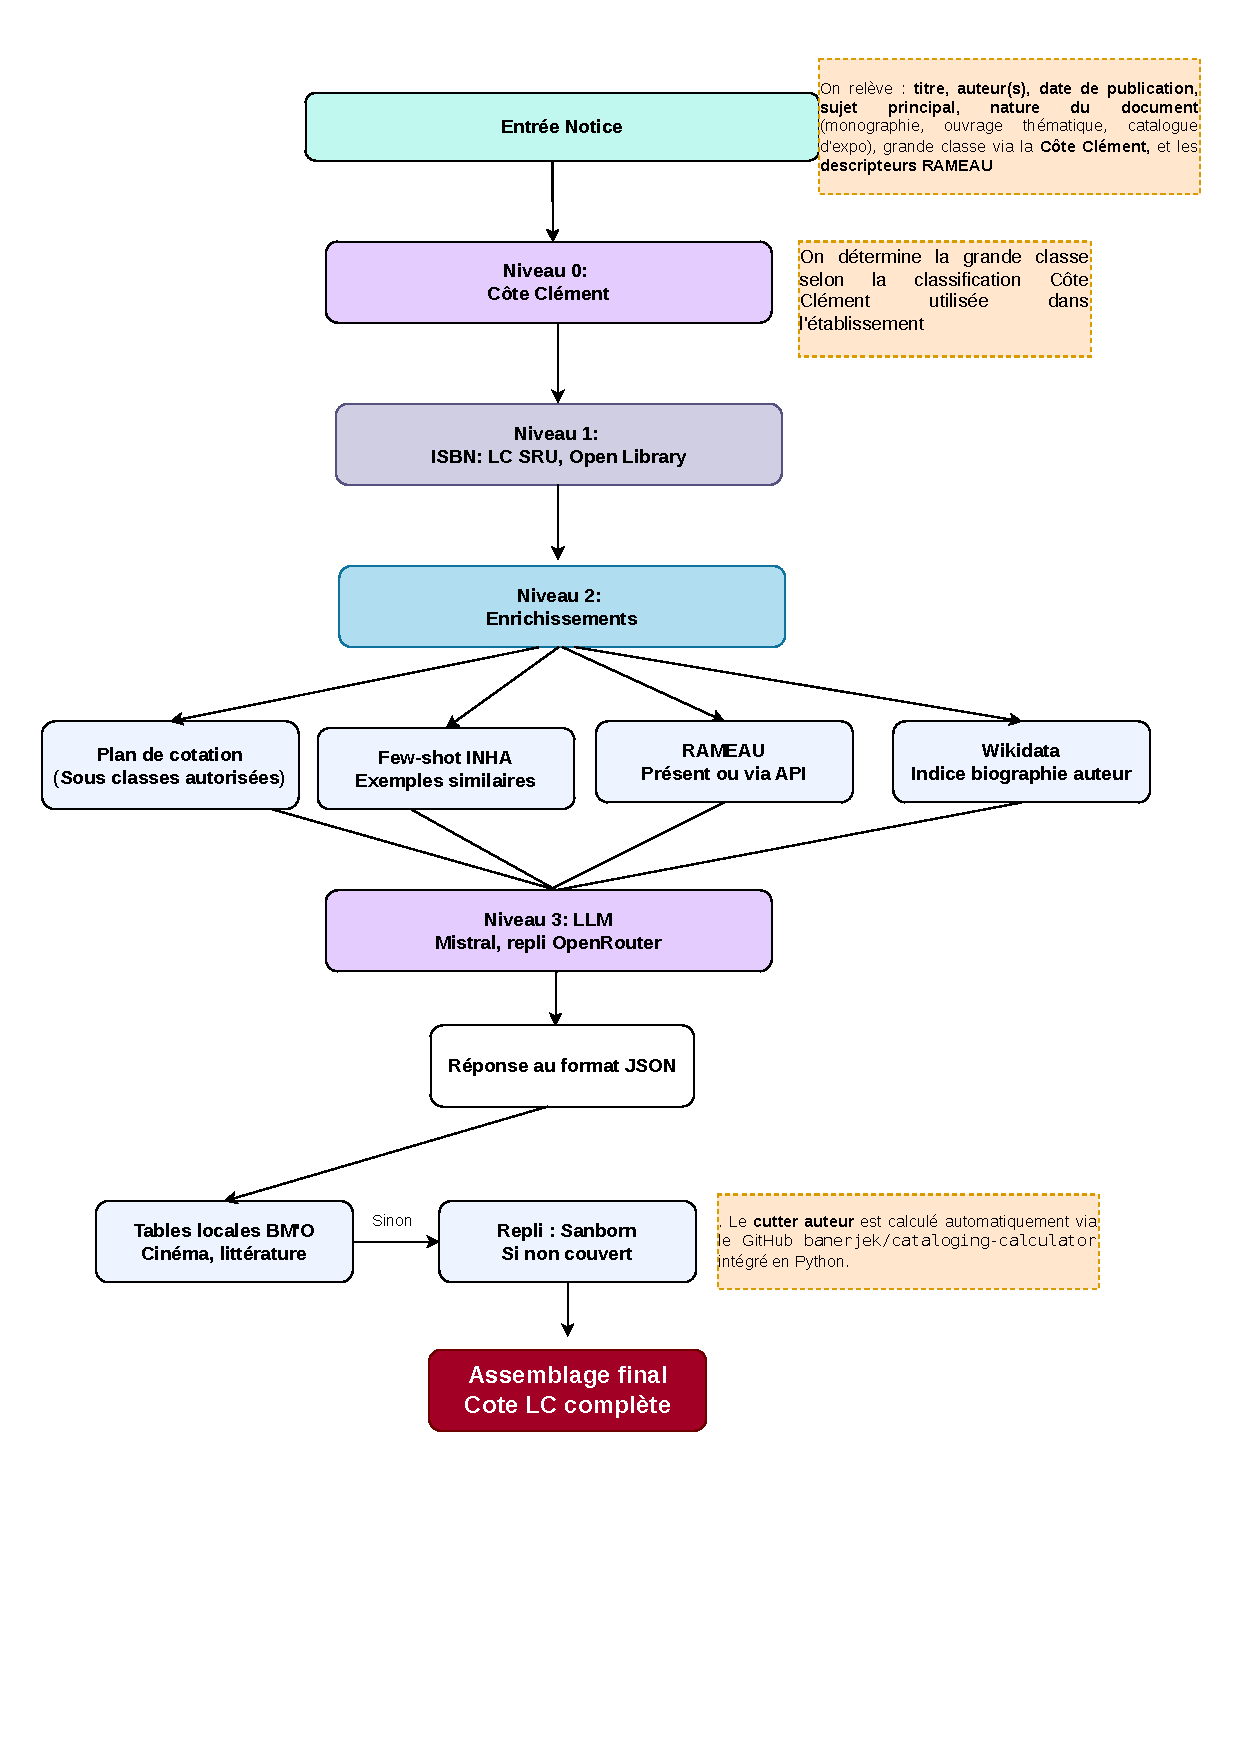
\includegraphics[width=0.85\textwidth]{schema_pipeline_cascade.pdf}%
  }
  \caption{Architecture du pipeline en cascade}
  \label{fig:pipeline}
\end{figure}


\subsection{Niveau 0 : grande classe via Cote Orsay interne}
\label{sec:niveau0}

Le \textit{pipeline}  de la cotation automatisée va se composer de plusieurs étapes successives. La première va consister en un simple dictionnaire pour déterminer la grande classe LC (par exemple, N pour les beaux-arts) à partir de la cote Orsay locale existante. Ce choix a été fait pour faciliter le travail du LLM et parce que c'était une étape qui pouvait être automatisée. La liste des grandes catégories est facilement traduisible en LCC.

Cette étape va restreindre le périmètre des classes autorisées dans le plan de cotation de la bibliothèque du musée d'Orsay et fournir au LLM un contexte cadré pour  choisir une sous-classe plus pertinente. La méthode est déterministe : la lettre Orsay (issue de la cotation locale) est traduite en grande classe \textit{Library of Congress} par une table de correspondance. Le coût en appel LLM est nul et ce socle déterministe est ce qui rend le reste du pipeline possible, puisqu'il libère les niveaux suivants de la charge d'identifier la grande classe pour se concentrer entièrement sur la sous-classe.

La difficulté ne se situe pas au niveau de la grande classe, où une étape conversion simple entre grandes classes est possible, mais au niveau de la sous-classe, là où la classification reste plus difficile à déterminer. C'est donc le LLM qui doit arbitrer entre la plausibilité formelle ou la pertinence sémantique. Ce choix a été fait pour exploiter l'ancienne cote Orsay locale, sécuriser la grande classe et concentrer l'effort de recherche là où se manifestent les limites de l'automatisation.





\begin{lstlisting}[caption={Extrait de la table de correspondance Cote Orsay (niveau 0)}, label={lst:correspondances}]
CORRESPONDANCES_ORSAY = {
    "P": "ND",   # Peinture
    "S": "NB",   # Sculpture
    "E": "N",    # Expositions
    "F": "TR",   # Photographie
    "UV": "AM",  # Musees
    # ...
}
\end{lstlisting}

\subsection{Niveau 1 : recherche par ISBN}
\label{sec:niveau1-isbn}

Une fois la première étape passée, c'est-à-dire la détermination de la grande classe, une deuxième étape vise à enrichir les données le plus possible avant de les fournir au LLM. Cette étape consiste à enrichir la notice d'information pour le LLM.

Elle repose sur l'interrogation de l'ISBN de l'ouvrage auprès de deux sources complémentaires : le service SRU de la \textit{Library of Congress}, puis, en cas d'échec, l'API Open Library.

Cette double interrogation nous donne une couverture combinée d'environ 48\%  des notices possédant un ISBN. 

Le choix de chercher l'ISBN s'appuie sur le script  de Melissa Belvadi\footcite{belvadi2023}, qui interroge les catalogues de Harvard, Stanford et Yale pour retrouver une cote LC déjà attribuée à un ISBN donné, avec un cache local SQLite évitant de solliciter inutilement les serveurs distants pour les ISBN déjà recherchés.



\subsection{Niveau 2 : enrichissement des métadonnées}
\label{sec:niveau2}


Dans la même logique que la recherche par ISBN, cette étape vise à enrichir les métadonnées de la notice avant de solliciter le LLM. Soit les sujets RAMEAU sont déjà présents dans les données initiales fournies à l'outil, soit ils sont recherchés via des appels API pour enrichir ces métadonnées. Une priorité est accordée aux sujets RAMEAU plutôt qu'au titre. Le titre peut en effet être trompeur : par exemple, un ouvrage intitulé « Musée Gaumont » peut traiter de cinéma et non de muséologie, tandis que les vedettes RAMEAU définissent les véritables sujets intellectuels de l'ouvrage.

Le plan de cotation est ensuite injecté dans le prompt. C'est un plan qui a été validé par l'équipe de la bibliothèque. Le LLM ne reçoit que les sous-classes de la grande classe déjà identifiées et extraites de ce plan. Deux sources l'alimentent : les plans détaillés fournis par l'équipe de la bibliothèque pour les domaines spécifiques et le plan générique LCC en JSON pour les autres domaines.


Cette étape d'enrichissement, dont nous testerons la validité, a pour objectif de donner le plus de chances possible au LLM de choisir la sous-classe la plus pertinente, grâce aux sujets RAMEAU et à l'enrichissement \textit{few-shots}.



\subsection{Niveau 3 : proposition par le LLM}
\label{sec:niveau3-llm}


Le \textit{pipeline}  utilise principalement le modèle Mistral NeMo comme fournisseur principal. Ce modèle a été retenu pour son accès facile et gratuit et sa disponibilité via une API REST\footnote{Une API REST (\textit{Representational State Transfer}) est un style d'architecture standard pour l'échange de données entre logiciels par le protocole HTTPS : chaque requête est autonome et transmise sous une forme normalisée, ce qui la rend indépendante du langage de programmation utilisé de part et d'autre.}.

Le recours à un LLM à ce niveau précis de la cascade, plutôt qu'à une méthode déterministe comme aux niveaux précédents, se justifie par la nature même de la tâche restante : le choix d'une sous-classe pertinente exige un jugement sémantique sur le contenu du document, pour lequel aucune règle simple ne suffit (voir §\ref{sec:justification-architecture}).

Le mécanisme de bascule fonctionne notice par notice, à la suite d'échecs de service rencontrés au cours du développement. Le pipeline tente d'abord Mistral et en cas d'échec distingue deux types d'erreurs. Des erreurs transitoires (comme un quota dépassé), qui déclenche une nouvelle tentative après un délai d'attente, et des erreurs définitives (authentification refusée, accès non autorisé au modèle), qui déclenche une bascule vers un autre fournisseur, OpenRouter. Si les deux fournisseurs échouent l'un après l'autre pour une même notice, le processus s'arrête en sauvegardant la notice.

Les deux services sont interrogés par appel HTTPS direct plutôt que par un kit de développement logiciel tiers (\textit{SDK}), pour trois raisons. Eviter d'installer et de maintenir une dépendance supplémentaire par fournisseur, alors que l'environnement Colab repart de zéro à chaque session. Ensuite, permettre de traiter Mistral et OpenRouter de façon strictement identique dans le code, avec un seul mécanisme de gestion des erreurs (voir plus haut), plutôt que d'adapter la logique de bascule à deux SDK différents, avec chacun ses propres conventions. Enfin, l'appel direct donne un accès complet et sans intermédiaire au code de statut et au contenu exact de chaque réponse, nécessaire comprendre les messages d'erreurs.


La température du modèle, le paramètre qui contrôle le degré de variation aléatoire dans la réponse générée, a été fixée à 0,1, une valeur assez basse. Cela signifie que pour une même notice interrogée plusieurs fois, le modèle produit des réponses identiques ou très proches.
C'est une condition nécessaire pour produire des résultats reproductibles d'une exécution à l'autre, et elle facilite le travail des bibliothécaires ou des personnes qui utilisent l'outil pour obtenir des résultats identiques pour chaque notice.
Le prompt envoyé au modèle assemble plusieurs éléments, chacun avec un but spécifique. D'abord, la grande classe est déjà connue : le modèle n'a pas à la déterminer, il doit juste choisir la sous-classe. Le plan des sous-classes lui est fourni au format CSV (reproduit en annexe) : c'est un plan spécifique déterminé par la bibliothèque du musée d'Orsay, qui délimite toutes les sous-classes possibles et restreint l'espace des réponses à un sous-ensemble pertinent, plutôt qu'à l'ensemble du plan \textit{Library of Congress}.

Ensuite, on appelle une API de l'INHA qui recherche les notices les plus proches par similarité de celle que l'on cherche à coter. On appelle cela du \textit{few-shot}, ce qui montre au modèle un motif concret plutôt qu'une règle abstraite. On lui fournit également une consigne explicite de prioriser les sujets RAMEAU plutôt que le titre. 

Le \textit{prompt}  demande enfin une réponse limitée à la seule cote au format JSON, afin qu'elle puisse être exploitée automatiquement dans la suite du \textit{pipeline} . Le LLM ne produit que la sous-classe : une décision prise pour se concentrer sur ce point plus sensible et plus sujet à l'erreur, plutôt que sur la grande classe.


\subsection{Justification des choix architecturaux}
\label{sec:justification-architecture}

\subsubsection*{L'architecture en cascade comme réponse aux limites des LLM}

L'idée de l'architecture du pipeline résulte d'une réponse aux limites des grands modèles de langage identifiées précédemment. Le but était de mettre en situation l'instruction générative  (\textit{prompting}) du LLM de bout en bout, mais le recours à un LLM sur l'architecture entière présenterait trois problèmes majeurs.

Le premier problème est d'ordre économique et temporel. Chaque appel à un LLM est coûteux, long et peut induire des erreurs si tout repose sur lui. À l'inverse, les niveaux déterministes précédant l'appel au LLM facilitent le travail et donnent plus de chances d'obtenir un résultat correct, plus rapide et moins coûteux. Sur un corpus de 50 000 notices, la différence est considérable.

Une logique de cascade va concentrer le traitement coûteux uniquement sur la partie la plus difficile, c'est-à-dire les étapes qu'on ne peut pas résoudre automatiquement. Cela rejoint un principe de conception bien ancré dans l'apprentissage automatique, notamment popularisé par les détecteurs en cascade \footcite{violajones2001}: plusieurs étapes de classifieurs, du moins coûteux au plus coûteux, filtrent progressivement les cas à traiter pour ne réserver le traitement complexe qu'à la minorité de cas non résolus précédemment. La différence est que les niveaux de ce pipeline de cotation répondent à des questions différentes (grande classe, cotes par ISBN, sous-classe) et fonctionnent plutôt comme une chaîne de méthodes de secours que comme un raffinement progressif. Mais le principe reste d'économiser le calcul coûteux en le réservant à l'étape la plus difficile.

Le second problème est la fiabilité. On peut utiliser la correspondance avec l'ancienne cotation Orsay pour prédire la grande classe, atteindre 100\% de justesse et ainsi augmenter la précision pour l'étape où le LLM doit trouver la sous-classe. Sans cette étape, un LLM, même contraint par un prompt, a plus de chances de générer des erreurs.

Le troisième problème est la traçabilité. L'architecture de ce \textit{pipeline}  est conçue pour attribuer à chaque côte une source explicite et un niveau de confiance numérique. Un LLM unique de bout en bout offre peu de fiabilité, surtout par \textit{prompting}, concernant l'origine de la réponse. La cascade permet de contraindre le LLM et ses erreurs à une seule étape, pour que l'utilisateur final sache à tout moment d'où vient la cote proposée.


\subsubsection*{Le fine-tuning écarté faute de ressources}
La possibilité d'utiliser le \textit{ fine-tuning}  du modèle au lieu du \textit{pipeline}  a été envisagée mais écartée. Les raisons de ce choix sont matérielles et méthodologiques : le corpus d'entraînement disponible est trop petit et insuffisant pour un \textit{ fine-tuning}  satisfaisant, et l'infrastructure ne dispose pas d'un GPU adapté à cette tâche.

Dans le cas de ce projet, la solution a donc été de s'orienter vers du  \textit{few-shot prompting}, qui constitue un compromis entre performance et contraintes. 


\subsubsection*{La dépendance aux API externes comme fragilité structurelle}

L'architecture du \textit{pipeline}  repose sur un nombre important de services externes : le SRU de la Library of Congress et Open Library pour l'enrichissement par ISBN, les API de recherche RAMEAU, l'API de similarité de l'INHA pour le \textit{few-shot}, et enfin les fournisseurs de LLM Mistral et OpenRouter. Cette multiplication des dépendances constitue une fragilité structurelle du \textit{pipeline}: chacun de ces services échappe au contrôle de la bibliothèque du musée d'Orsay, que ce soit en matière de disponibilité, de quota, de changement de format de réponse ou de suppression pure et simple du service, comme cela a déjà été observé lors des tests de plusieurs sources d'enrichissement par ISBN écartées en cours de projet.

Cette fragilité est d'autant plus sensible que le corpus à traiter est volumineux : sur 50 000 notices, une indisponibilité même brève d'un service peut interrompre un traitement de plusieurs heures. Pour limiter ce risque, un mécanisme de disjoncteur (\emph{circuit breaker}) a été intégré à la boucle de traitement : après cinq échecs consécutifs d'un même service, le pipeline enregistre un point de sauvegarde et interrompt l'exécution plutôt que de poursuivre sur des données dégradées ou de saturer inutilement le service distant. Ce choix ne supprime pas la dépendance, mais il permet de reprendre le traitement là où il s'est arrêté plutôt que de perdre l'intégralité d'une exécution.

Cette architecture pose donc une limite méthodologique à anticiper pour tout déploiement en production : la robustesse du \textit{pipeline}  dans la durée dépendra autant de la stabilité des API tierces que de la qualité du code lui-même.

\subsubsection*{La priorisation RAMEAU, levier puissant mais fragile}

Parmi les enrichissements testés, la priorisation des sujets RAMEAU sur le titre de l'ouvrage semble être le levier le plus déterminant pour orienter le LLM vers la sous-classe pertinente. La nature même du champ RAMEAU,  informe sur le sujet intellectuel  de l'ouvrage, quand le titre peut être trompeur ou allusif.

Ce levier reste toutefois fragile pour deux raisons. D'une part, la qualité du champ RAMEAU est hétérogène d'une notice à l'autre : certaines notices disposent de sujets RAMEAU précises et nombreuses, d'autres sont lacunaires ou absentes, ce qui limite mécaniquement le bénéfice de la priorisation aux seules notices correctement indexées. D'autre part, la performance du \textit{pipeline}  sur ce point dépend directement de la qualité du catalogage antérieur réalisé par la bibliothèque, un facteur externe au \textit{pipeline}  lui-même et non maîtrisable par l'automatisation. Un enrichissement RAMEAU de meilleure qualité en amont, ou une politique de catalogage plus systématique, aurait donc un effet direct sur la performance du \textit{pipeline} , indépendamment de toute amélioration technique de la cascade elle-même.

Cette fragilité illustre une limite plus générale de l'automatisation par LLM dans ce contexte : le \textit{pipeline}  ne peut pas compenser entièrement un déficit de métadonnées structurées en amont, il ne peut qu'exploiter au mieux ce qui est disponible.

\section{Constitution du corpus de référence et limites de la validation}

\subsection{L'absence de vérité terrain à Orsay}
\label{sec:absence-verite-terrain}

Une des réponses apportées à cette contrainte a été de recourir à un corpus provenant de l’INHA, qui a recoté une partie de ses collections au format Library of Congress. Le choix méthodologique retenu pour ce corpus est d’imposer la grande classe telle qu’elle figure dans la cote INHA de référence, plutôt que de la faire dériver du niveau 0 du pipeline (\S\ref{sec:niveau0}) : les notices INHA ne portent pas de Cote Orsay, ce niveau ne peut donc pas y être exercé. Ce choix permet de concentrer l’évaluation sur ce que ce corpus peut effectivement mesurer, à savoir la qualité de la sous-classe proposée par le LLM et l’apport des enrichissements de la cascade, mais il a une conséquence qu’il faut garder à l’esprit dans la lecture des résultats de la Partie 3 : la justesse de la correspondance cote Orsay → grande classe elle-même n’est testée par aucune de ces expériences, et les scores obtenus sur ce corpus ne mesurent donc que le comportement du LLM en aval d’une grande classe supposée correcte, pas la performance de bout en bout du pipeline sur un fonds réel.

L’utilisation du corpus de l’INHA comme banc d’essai présente toutefois des limites qu’il convient de lister. L’INHA a en effet adapté la Library of Congress à ses propres règles et appliqué sa propre politique de cotation, qui diverge des choix retenus à Orsay ainsi que de la cotation classique de la Library of Congress. 

Notamment, elle regroupe sous des sous-classes locales NY et NZ, qui n'existent pas dans la \textit{Library of Congress Classification}, l'ensemble des documents portant sur un même artiste quel qu'en soit le type (écrits et correspondance, catalogues raisonnés, monographies, catalogues d'exposition)\footcite{inhalcc}. 
L'organisation du libre accès en corpus thématiques y a été définie avant la correspondance avec la LCC, et c'est cette dernière qui a été adaptée en conséquence plutôt que l'inverse\footcite{inhalcc}. Les indices attribués par les bibliothèques américaines dont proviennent une partie des notices ne correspondent pas toujours aux classes retenues par l'INHA pour ses propres corpus, ce qui a nécessité des règles de correspondance locales~: des ouvrages sur le christianisme dans son rapport à l'esthétique, normalement classés en religion (BR115.A8), ont ainsi été réorientés vers la section Art (N72.R4)~; une partie des ouvrages sur l'histoire du vêtement, relevant en LCC de la classe Coutumes et folklore (GT), a été reclassée dans les Arts décoratifs (NK), section consacrée à la mode\footcite{inhalcc}. Ces réorientations sont motivées par la cohérence des corpus documentaires de l'INHA plutôt que par la logique disciplinaire de la LCC elle-même. 

 Les cotes \textit{Library of Congress}  de l’INHA ne constituent donc pas une vérité de terrain absolue. D’ailleurs, aucune cote ne constitue une vérité de terrain absolue. Le choix de l’INHA s’est fait en raison de la proximité de ses collections d’art avec celles de la bibliothèque du musée d’Orsay. 
Mais chaque bibliothèque a une politique et une approche différentes pour  établir ses cotes \textit{Library of Congress} , ce qui explique la complexité d’effectuer cette cotation.
Les choix de catalogage sont propres aux institutions, et parfois même au bibliothécaire lui-même, qui juge ce qui est optimal pour ses propres collections.

Le banc d’essai a été étendu depuis les premiers tests. Le corpus de l’INHA est désormais composé d’environ 200 notices couvrant une quinzaine de grandes classes, avec un sous-échantillon portant explicitement sur les 18 classes validées par la bibliothèque du musée d’Orsay. Cet élargissement permet d’assurer une meilleure robustesse statistique et de mettre en évidence un écart de performance potentiel entre les classes couvertes et non couvertes par le plan.


\section{Cadre d'évaluation : le degré de rapprochement}

\subsection{Pourquoi une évaluation binaire est insuffisante}
Dans le cadre de l'évaluation, le constat de départ est empirique. Proposer une cote ND 1345 alors que la cote attendue est ND 1350 n'est pas une erreur aussi grande que de proposer une grande catégorie TR au lieu de ND (TR correspondant à la photographie et ND à la peinture). Dans le premier cas, les deux cotes se situent dans la même catégorie, les paysages, alors que la seconde est une branche complètement différente de l'histoire de l'art.

Une évaluation binaire, c'est-à-dire savoir si la cote est strictement correcte ou non, serait donc une mauvaise manière d'interpréter les résultats. Une évaluation binaire nous donnerait peu d'informations sur le potentiel du LLM, notamment parce que la classification dépend des choix arbitraires du bibliothécaire et de l'institution, mais aussi parce qu'elle traiterait ces deux erreurs à la même échelle.

La classification de texte possède une structure hiérarchique de type arbre : une grande classe, une sous-classe, puis une cote précise. Comme l'a souligné la littérature sur les métriques d'évaluation de classification hiérarchique, une métrique qui ignore la hiérarchie mesure mal la qualité de la prédiction et masque le degré de rapprochement entre la cote attendue et la cote réelle\footcite{kosmopoulos2015,kiritchenko2006}.



\subsection{La distance au plus proche ancêtre commun}
\label{sec:distance-lca}

La méthode choisie dans ce pipeline a été d'établir un score qui va mesurer le degré de rapprochement hiérarchique entre la cote proposée et la cote de référence. Pour cela, on identifie, dans le barème LCC officiel complet (soit environ 497 préfixes de classe en hiérarchie parent-enfant, reconstituée à partir des barèmes PDF originaux de la \textit{Library of Congress}), le nœud le plus spécifique contenant chacune des deux sous-classes, puis on remonte leurs ancêtres jusqu'au plus proche ancêtre commun (\textit{lowest common ancestor},LCA).

La taille de cet intervalle est rapportée à l'étendue totale de la classe, ce qui donne une distance $d$ comprise entre 0 (sous-classes identiques) et 1 (aucun ancêtre commun spécifique au sein d'une même grande classe). 

Cette distance $d$ est ensuite convertie en un score de proximité sur une échelle de 0 à 4, par la formule $\text{score} = 4 \times (1 - d)$.Un score de 4,0 correspond à une sous-classe strictement exacte ($d = 0$), tandis qu'un score proche de 0 traduit une sous-classe hiérarchiquement très éloignée (dans la même grande classe). Lorsque la grande classe proposée diffère de la grande classe attendue, le score est fixé directement à 0,0, sans passer par le calcul de la distance LCA : cette situation est jugée qualitativement différente d'un simple éloignement de sous-classe, puisqu'elle correspond à une branche entièrement distincte de la classification (cf. l'exemple TR/ND en \S\ref{sec:niveau2}).

Le cutter est explicitement exclu de cette mesure : une fois la sous-classe déterminée, le calcul du cutter est une opération mécanique qu'il n'est pas nécessaire d'évaluer sur son inexactitude.




\begin{table}[h]
\centering
\begin{tabular}{ll}
\toprule
\textbf{Score} & \textbf{Signification} \\
\midrule
4,0 & Sous-classe exacte ($d = 0$) \\
$]0\,;\,4[$ & Proximité continue, $\text{score} = 4 \times (1 - d)$ \\
0,0 & Grande classe différente (distance LCA non calculée) \\
\bottomrule
\end{tabular}
\caption{Score de proximité de sous-classe, dérivé de la distance normalisée au plus proche ancêtre commun ($d$)}
\label{tab:score-lca}
\end{table}

\subsection{Méthodologie statistique}
\label{sec:methodologie-stats}

Les comparaisons entre conditions présentées en Partie 3 reposent sur trois outils statistiques, définis ici.

Le test de \textbf{Wilcoxon signé} (\textit{Wilcoxon signed-rank test})\footcite{wilcoxon1945} est un test non paramétrique adapté aux comparaisons appariées~: la même notice, évaluée dans deux conditions différentes. Il compare les rangs des différences observées entre les deux séries plutôt que leurs moyennes directement, ce qui le rend robuste à des distributions non normales (nos résultats étant bimodaux\S\ref{sec:distribution-score}). Un écart est considéré comme significatif au seuil nominal lorsque $p < 0{,}05$.

Les \textbf{intervalles de confiance par bootstrap}\footcite{efron1979} sont utilisés pour les scores par grande classe, où l'effectif est restreint. La méthode ré-échantillonne aléatoirement, avec remise, les scores observés d'une classe (2~000 itérations), pour estimer la variabilité de la moyenne sans supposer une loi de distribution connue. Un intervalle qui ne contient pas zéro indique un écart statistiquement établi~; un intervalle qui contient zéro signale un écart trop faible, ou un effectif trop réduit, pour être distingué du hasard de l'échantillonnage.


\section{Protocole expérimental}

\subsection{Vue d'ensemble des expériences}
\label{sec:vue-ensemble-experiences}

Le protocole isole l'effet de chaque levier de la cascade selon un plan factoriel~: deux plans de cotation (réduit BM'O, officiel complet) croisés avec quatre conditions d'enrichissement, soit huit configurations testées sur le même corpus de 201 notices. Le notebook fourni en annexe présente l'outil de cotation dans sa version de production~; les données brutes issues de l'exécution de ces huit configurations (score par notice et par configuration testée) sont fournies séparément au format CSV, et ont servi de base à l'ensemble des résultats et tests statistiques présentés en Partie 3.

\begin{table}[h]
\centering
\small
\setlength{\tabcolsep}{4pt}
\renewcommand{\arraystretch}{1.15}
\begin{tabular}{@{}p{0.15\textwidth}p{0.40\textwidth}p{0.40\textwidth}@{}}
\toprule
\textbf{Condition} & \textbf{Ce qui change par rapport à la configuration standard} & \textbf{Ce qui est mesuré} \\
\midrule
Standard           & RAMEAU actif, few-shot actif (pool de 26 notices) & Configuration de référence \\
RAMEAU désactivé   & Sujets RAMEAU retirés du \textit{prompt}          & Effet de la priorisation RAMEAU (Partie~3, \S\ref{sec:effet-rameau}) \\
Few-shot désactivé & Aucun exemple fourni au modèle                    & Effet du \gls{fewshot} (Partie~3, \S\ref{sec:effet-fewshot}) \\
Pool élargi        & Pool few-shot porté de 26 à 94 notices            & Effet de la taille du pool (Partie~3, \S\ref{sec:effet-pool-elargi}) \\
\bottomrule
\end{tabular}
\caption{Les quatre conditions testées, chacune sous plan réduit et sous plan officiel complet}
\label{tab:experiences}
\end{table}


Chaque condition isole un seul levier à la fois par rapport à la configuration standard, plutôt que de les cumuler progressivement~: cela permet de mesurer l'effet propre de chaque enrichissement, y compris ses variations selon le plan de cotation utilisé (Partie 3, \S\ref{sec:effet-plan-reduit}), plutôt qu'un effet confondu avec l'ordre dans lequel les leviers auraient été ajoutés.

Le détail du test opposant le plan réduit de la bibliothèque du musée d'Orsay au barème LCC complet est présenté et discuté en Partie 3, \S\ref{sec:effet-plan-reduit}, à partir des données brutes fournies en annexe.


\part{Résultats, discussion et \textit{workflow} proposé}
% !TEX root = memoire.tex
% !BIB program = biber

\chapter{Résultats, discussion et proposition de workflow}
\label{chap:partie3}


\section{Résultats}
\label{sec:resultats}

\subsection{Généralisation multi-classes}
\label{sec:generalisation-multiclasses}

\subsubsection*{Score global}
\label{sec:score-global}

Pour un corpus de $n = 201$ notices, en configuration standard (\gls{rameau} activé, plan de la bibliothèque du musée d'Orsay (BM'O) réduit, exemples \gls{inha}), le \textit{pipeline} atteint un score micro-moyen de 2,394/4 et un taux d'exact-match de 59,2~\% sur les sous-classes. Ces chiffres, comme l'ensemble de ceux présentés dans ce chapitre, sont mesurés sur le corpus de substitution INHA et sa politique de cotation propre (Partie 2, §\ref{sec:absence-verite-terrain}) ; ils caractérisent le comportement du \textit{pipeline} sur ce banc d'essai, pas une performance mesurée sur le fonds réel de la BM'O.

Le score micro-moyen est calculé sur l'ensemble des notices prises individuellement, ce qui le rapproche mécaniquement de la performance des classes les plus peuplées ; le score macro-moyen, à l'inverse, est la moyenne des scores par classe, indépendamment de son effectif. Le score macro-moyen s'établit à 2,309/4. Cet écart entre score micro et macro s'explique par une forte hétérogénéité de la performance selon les classes.

\begin{table}[h]
\centering
\begin{tabular}{lrrrl}
\toprule
\textbf{Grande classe} & \textbf{$n$} & \textbf{Score moyen (/4)} & \textbf{Exact-match} & \textbf{IC 95~\%} \\
\midrule
NK (Arts décoratifs)        & 27 & 3,46 & 85,2~\% & [2,92 ;~3,91] \\
AM (Musées, collections)    & 43 & 3,26 & 81,4~\% & [2,79 ;~3,72] \\
NX (Arts, généralités)      & 15 & 2,40 & 60,0~\% & [1,33 ;~3,47] \\
NA (Architecture)           & 33 & 2,30 & 57,6~\% & [1,58 ;~2,91] \\
N (Beaux-arts, généralités) & 55 & 1,38 & 34,5~\% & [0,87 ;~1,89] \\
\bottomrule
\end{tabular}
\caption{Score par grande classe, configuration standard ($n \geq 10$, intervalle de confiance \textit{bootstrap}  à 95~\%)}
\label{tab:score-grande-classe}
\end{table}

L'écart entre classes est net et se maintient sur l'ensemble des expérimentations menées dans ce chapitre~: NK et AM dépassent 80~\% d'exact-match, tandis que N plafonne à 34,5~\%. Cette dernière est aussi la classe la plus peuplée du corpus, avec un effectif de 55 notices, ce qui pèse fortement sur le score micro-moyen. Les causes de cette hétérogénéité : sensibilité au plan de cotation, effet de la priorisation RAMEAU, effet d'attracteur propre à certaines classes, sont examinées successivement dans les sections qui suivent (\S\ref{sec:effet-plan-reduit}, \S\ref{sec:effet-rameau}, \S\ref{sec:taxonomie-erreurs}).

\subsection{Distribution du score continu}
\label{sec:distribution-score}

Le score de proximité utilisé dans ce mémoire est continu, gradué de 0 à 4 selon la distance au plus proche ancêtre commun dans le barème. Cette granularité avait pour but de distinguer, parmi les erreurs, celles qui restent proches de la sous-classe attendue de celles qui en sont très éloignées.

\begin{table}[h]
\centering
\begin{tabular}{lc}
\toprule
\textbf{Tranche de score} & \textbf{Part des notices} \\
\midrule
0 (aucun ancêtre commun) & 39,8~\% \\
]0 -- 1] éloigné & 0,0~\% \\
]1 -- 2] proche & 0,5~\% \\
]2 -- 3] très proche & 0,0~\% \\
]3 -- 4] quasi exact / exact & 59,7~\% \\
\bottomrule
\end{tabular}
\caption{Distribution du score de proximité, configuration standard (n = 201)}
\label{tab:distribution-score}
\end{table}

Dans les faits, cette gradation se révèle peu exploitée par les résultats obtenus. La distribution est fortement bimodale~: 39,8~\% des notices obtiennent un score nul et 59,7~\% un score quasi exact ou exact, tandis que les tranches intermédiaires représentent ensemble moins de 1~\% du corpus. Le modèle ne s'approche donc que très rarement de la bonne réponse sans l'atteindre~: soit il identifie directement la sous-classe attendue ou une sous-classe très proche, soit il en propose une sans lien hiérarchique avec elle.

Cette bimodalité a deux conséquences pour la lecture de ce chapitre. D'une part, le score continu et le taux d'exact-match mesurent, sur ce corpus, presque la même chose. D'autre part, elle rend difficile de distinguer ce qui relève du comportement du modèle et ce qui relève de la granularité du barème utilisé pour la mesure, une question discutée en \S\ref{sec:limites}.




\subsection{Effet du plan de cotation}
\label{sec:effet-plan-reduit}

\subsubsection*{Hypothèse et protocole}

L'un des tests les plus importants de ce corpus est celui de l'effet de la taille du plan de cotation. Dans ce test, on observe les conséquences des restrictions de l'espace des sous-classes proposées au \gls{llm}.

On compare les résultats obtenus avec le plan de cotation restreint par la bibliothèque du musée d'Orsay et le barème officiel LCC complet extrait des \textit{schedule} de la \textit{Library of Congress}. La différence est de plusieurs milliers d'entrées par classe pour le barème officiel, contre quelques dizaines pour le plan réduit.
Sur les 201 notices de corpus, on a deux conditions de comparaison qui ont été testées en ce qu'on va appeler configuration standard avec les enrichissements RAMEAU et \textit{few-shot}. 


\begin{table}[h]
\centering
\begin{tabular}{lccl}
\toprule
\textbf{Condition} & \textbf{Score moyen} & \textbf{Exact-match} & \textbf{p (Wilcoxon)} \\
\midrule
Plan réduit, config. standard & 2,394 & 59,2~\% & \multirow{2}{*}{0,038} \\
Plan officiel, config. standard & 1,917 & 45,3~\% & \\
\midrule
Plan réduit, few-shot désactivé & 2,673 & 66,2~\% & \multirow{2}{*}{$1,6\times10^{-5}$ \textbf{(Bonferroni)}} \\
Plan officiel, \textit{few-shot} désactivé & 1,823 & 43,3~\% & \\
\bottomrule
\end{tabular}
\caption{Effet du plan de cotation, sous deux conditions de \textit{few-shot} (n = 201)}
\label{tab:plan-reduit-officiel}
\end{table}

Dans cette configuration standard, on obtient un résultat de 64 notices qui obtiennent un meilleur score avec le plan restreint de la bibliothèque du musée d'Orsay, contre 37 qui se dégradent et 100 qui restent inchangées. Le solde net est donc positif, soit un solde net positif de 27 notices en faveur du plan réduit, donc 13,4\% du corpus.

On utilise un test statistique pour vérifier la significativité des résultats, le test de \gls{wilcoxon}. 
Ce test confirme la significativité de cet écart. Pour lire ce test, le p doit être inférieur à 0,05.


Lorsque le \textit{few-shot} est désactivé, la même comparaison donne un écart plus large et plus observable. 71 notices vont s'améliorer sous le plan réduit contre 26 qui se dégradent et 104 sont inchangées, soit un solde net de 45 notices.
Le score net passe de 2,673 sur le plan réduit à 1,823 sur le plan officiel, un gain de 0,850 point, et l'exact match passe de 66,2\% sous le plan réduit à 43,3\% sous plan officiel et donc une chute de 22,9 points.

On peut conclure que dans ces conditions, le plan réduit obtient une meilleure performance que le plan officiel dans la majorité des classes du corpus avec un écart plus marqué en l'absence du \textit{few-shot}. 64 notices améliorées contre 37 en configuration standard et 71 contre 26 en \textit{few-shot} désactivé.

Cette tendance n'est pas universelle. On observe une tendance différente dans les résultats de la classe N.

\subsubsection*{Hétérogénéité par grande classe}

L'effet de cette tendance n'est pas homogène et, dans certains cas, sa direction s'inverse.
Le tableau ci-dessous détaille les scores moyens obtenus pour chaque plan pour les classes dont l'effectif dépasse 7 notices, c'est-à-dire 180 sur 201 notices du corpus, et les 21 restantes sont un peu trop peu représentées pour un score fiable. Ces échantillons sont d'effectifs réduits.


\begin{table}[h]
\centering
\begin{tabular}{lcccc}
\toprule
\textbf{Grande classe} & \textbf{n} & \textbf{Plan réduit} &
\textbf{Plan officiel} & \textbf{Écart [IC 95\,\%]} \\
\midrule
NK (Arts décoratifs)          & 27 & 3,46 & 0,68 & $+2{,}78$ $[+2{,}17\,;\,+3{,}32]$ \\
AM (Musées, collections)      & 43 & 3,26 & 1,95 & $+1{,}31$ $[+0{,}56\,;\,+2{,}05]$ \\
NX (Arts, généralités)        & 15 & 2,40 & 1,67 & $+0{,}73$ $[-0{,}80\,;\,+2{,}33]$ \\
ND (Peinture)                 &  7 & 2,83 & 2,26 & $+0{,}57$ $[-1{,}14\,;\,+2{,}29]$ \\
NA (Architecture)             & 33 & 2,30 & 2,37 & $-0{,}07$ $[-0{,}85\,;\,+0{,}73]$ \\
N  (Beaux-arts, généralités)  & 55 & 1,38 & 2,25 & $-0{,}87$ $[-1{,}45\,;\,-0{,}29]$ \\
\bottomrule
\end{tabular}
\caption{Score moyen par grande classe, plan réduit vs plan officiel.}
\label{tab:plan-par-classe}
\end{table}

On va utiliser un intervalle de confiance à 95\% par \textit{bootstrap}.Avec ces résultats, on observe que deux classes bénéficient du plan réduit de façon statistiquement établie : la classe NK (Arts décoratifs) + 69\% du score maximal et AM (Musées, collections) + 32\%. Ce sont les deux classes qui sont les plus impactées par la réduction du plan.

Deux autres classes ont un effectif plus restreint qui ne permet pas de conclure à un effet statistiquement établi, mais suggère un effet favorable au plan réduit : NX (Arts, généralités, +18\%) et ND (Peinture + 14\%).

Deux classes vont faire exception : NA (Architecture) reste stable entre les deux plans et la classe N (Beaux-arts, généralités) a un résultat inverse et significatif. Elle obtient un meilleur score avec le plan officiel, soit un écart de 21,8\% en faveur de celui-ci.
Une hypothèse de cette différence est celle de l'effet d'attraction sur une plage du plan réduit mal définie pour cette classe.

\subsubsection*{Exemple qualitatif}

Pour la notice \emph{Costume}, par Louise Alcan et Michèle Margerie (cote réelle \texttt{AM48.P37~T73~1983}), le plan réduit guide correctement le modèle vers la tranche \texttt{AM10-100} (\textit{By country}, score~4). Le plan officiel complet propose \texttt{AM349}, une cote qui relève de la sous-section \textit{Collectors and collecting} (\texttt{AM200-501}) dédiée aux collectionneurs privés et à leurs pratiques plutôt que de la sous-section \textit{By country} (\texttt{AM10-100}) qui décrit les musées nationaux et leurs collections. Ce choix aboutit à un score nul. C'est un exemple de dispersion du modèle dans un espace de réponses nettement plus large.

\subsection{Effet de la priorisation RAMEAU}
\label{sec:effet-rameau}

Ce test a pour but de quantifier l'apport de la consigne LLM de prioriser les vedettes RAMEAU de la notice plutôt que le titre pour déterminer la sous-classe, dans la logique où le titre peut être trompeur.

\begin{table}[h]
\centering
\begin{tabular}{lccl}
\toprule
& \textbf{Score moyen} & \textbf{Exact-match} & \textbf{p (Wilcoxon)} \\
\midrule
RAMEAU activé, plan réduit & 2,394 & 59,2~\% & \multirow{2}{*}{0,0035 \textbf{(Bonferroni)}} \\
RAMEAU désactivé, plan réduit & 2,076 & 51,2~\% & \\
\midrule
RAMEAU activé, plan complet & 1,917 & 45,3~\% & \multirow{2}{*}{0,238} \\
RAMEAU désactivé, plan complet & 1,791 & 41,8~\% & \\
\bottomrule
\end{tabular}
\caption{Effet de la priorisation RAMEAU, sous les deux plans (n = 201)}
\label{tab:rameau-on-off}
\end{table}


On observe que la priorisation des sujets RAMEAU sur le titre améliore significativement les résultats sous plan réduit. On a une amélioration de 8\% du score maximal. C'est l'un des deux seuls effets de ce mémoire à résister à la correction de Bonferroni.

Sous plan officiel, cet effet s'atténue fortement et perd sa significativité. On obtient seulement un gain de 3,2\%.

Ces résultats montrent que l'ajout de l'importance des sujets RAMEAU dépend de la taille de l'espace des réponses. Elles semblent plus utiles lorsque le modèle dispose de moins d'informations et d'un espace restreint et se dilue face à la difficulté générale de navigation du LLM dans un espace de plusieurs milliers d'options.

\subsubsection*{Hétérogénéité par grande classe}

\begin{table}[h]
\centering
\begin{tabular}{lcccc}
\toprule
\textbf{Grande classe} & \textbf{n} & \textbf{Écart moyen} & \textbf{IC 95\%} & \textbf{Robuste ?} \\
\midrule
N (Beaux-arts, généralités) & 55 & $+0{,}44$ & [$+0{,}15$ ; $+0{,}80$] & \textbf{Oui} \\
NK (Arts décoratifs) & 27 & $+0{,}44$ & [$0{,}00$ ; $+0{,}89$] & Non \\
NX (Arts, généralités) & 15 & $+0{,}27$ & [$0{,}00$ ; $+0{,}80$] & Non \\
AM (Musées, collections) & 43 & $+0{,}09$ & [$-0{,}56$ ; $+0{,}74$] & Non \\
NA (Architecture) & 33 & $+0{,}00$ & [$-0{,}36$ ; $+0{,}36$] & Non \\
\bottomrule
\end{tabular}
\caption{Écart de score RAMEAU on/off par grande classe, IC bootstrap 95\% (plan réduit)}
\label{tab:rameau-par-classe}
\end{table}

C'est la classe N, et non une classe à meilleure performance globale, qui porte l'essentiel de l'effet RAMEAU mesuré au niveau global~: c'est la seule classe dont l'intervalle de confiance ne contient pas zéro. Pour NK, NX, AM et NA, les intervalles incluent zéro et ne permettent pas d'établir un effet propre à ces classes sur cet échantillon. RAMEAU pourrait ainsi agir, sur la classe la plus difficile du corpus, comme un signal suffisamment spécifique pour contrer le repli par défaut du modèle vers sa zone d'attraction.

\subsection{Effet du few-shot}
\label{sec:effet-fewshot}

\begin{table}[h]
\centering
\begin{tabular}{lccl}
\toprule
& \textbf{Score moyen} & \textbf{Exact-match} & \textbf{p (Wilcoxon)} \\
\midrule
Few-shot activé, plan réduit & 2,394 & 59,2~\% & \multirow{2}{*}{0,027} \\
Few-shot désactivé, plan réduit & 2,673 & 66,2~\% & \\
\midrule
Few-shot activé, plan complet & 1,917 & 45,3~\% & \multirow{2}{*}{0,376} \\
Few-shot désactivé, plan complet & 1,823 & 43,3~\% & \\
\bottomrule
\end{tabular}
\caption{Effet du few-shot, sous les deux plans (n = 201)}
\label{tab:fewshot-on-off}
\end{table}

Contrairement à l'hypothèse initiale de ce mémoire, ajouter des exemples \textit{few-shot} au prompt \textbf{dégrade} les résultats sous plan réduit~: les retirer améliore le score plutôt que de le détériorer ($-0{,}279$, $p=0{,}027$). \textbf{La meilleure configuration mesurée dans ce mémoire, toutes conditions confondues, est donc le plan réduit sans few-shot} (2,673, 66,2~\% d'exact-match), et non le plan réduit avec few-shot activé. Sous plan officiel complet, l'effet s'inverse et redevient légèrement positif, sans significativité ($+0{,}094$, $p=0{,}376$)~: lorsque l'espace de réponses est déjà restreint et pertinent, les exemples n'apportent pas d'information supplémentaire utile et semblent détourner le modèle d'un raisonnement direct à partir du plan fourni.

\subsection{Effet du pool \textit{few-shot} élargi}
\label{sec:effet-pool-elargi}

Le pool \textit{few-shot} original ne compte que 26 notices de référence. Un corpus élargi à 94 notices, constitué à partir de notices INHA non utilisées, a été testé pour vérifier si cet effectif restreint limitait l'effet de guidage du modèle.

\begin{table}[h]
\centering
\begin{tabular}{lccl}
\toprule
& \textbf{Score moyen} & \textbf{Exact-match} & \textbf{p (Wilcoxon)} \\
\midrule
Pool original (26), plan réduit & 2,394 & 59,2~\% & \multirow{2}{*}{0,354} \\
Pool élargi (94), plan réduit   & 2,534 & 62,7~\% & \\
\midrule
Pool original (26), plan complet & 1,917 & 45,3~\% & \multirow{2}{*}{0,014} \\
Pool élargi (94), plan complet   & 2,369 & 58,2~\% & \\
\bottomrule
\end{tabular}
\caption{Score moyen selon la taille du pool few-shot, sous les deux plans (n = 201)}
\label{tab:fewshot-pool}
\end{table}

L'effet du corpus élargi est asymétrique selon le plan de cotation~: sous plan réduit, le gain reste modeste et non significatif ($+0{,}139$, $p=0{,}354$) ; sous plan complet, il devient net ($+0{,}451$, $p=0{,}014$, significatif mais non robuste au seuil de Bonferroni).

Toutefois, ces résultats doivent prendre en compte l'hétérogénéité des classes. Pour la classe NX, le score se dégrade avec le corpus élargi~: il passe de 2,40 (corpus original) à 1,87 (corpus élargi) sous plan réduit, l'exact-match chutant de 60,0~\% à 46,7~\%.

Le corpus élargi comptant une forte proportion de notices de la classe N (majoritaire dans le corpus source) contre très peu de notices NX, cette composition déséquilibrée tend à réintroduire, pour les classes minoritaires du pool, un biais de représentation hérité du corpus dont il est issu.

Une amélioration future de la méthode few-shot serait de privilégier un élargissement homogène, avec des exemples pour toutes les classes.

\subsection{Taxonomie des erreurs}
\label{sec:taxonomie-erreurs}

\subsubsection*{Une attraction vers une cote mal différenciée}

Une observation plus poussée sur les prédictions de la classe N révèle qu'une part importante des notices se voient attribuer exactement la même cote \texttt{N7560-8266}, indépendamment du sujet réel, y compris pour des ouvrages portant le terme baroque  dans leur titre (qui devraient relever de \texttt{N6415.B3}). Cette cote correspond, dans le plan réduit BM'O, à une entrée unique regroupant les sujets spéciaux de l'art, alors qu'elle est subdivisée en plusieurs dizaines d'entrées distinctes dans le plan officiel complet.

\begin{table}[h]
\centering
\begin{tabular}{lccc}
\toprule
& \textbf{Notices recevant} & \textbf{Part} & \textbf{Score moyen} \\
& \textbf{la cote \texttt{N7560-8266}} & \textbf{(/55)} & \textbf{(/4)} \\
\midrule
Plan réduit (BM'O)      & 20/55 & 36,4~\% & 1,38 \\
Plan officiel (complet) & 0/55  & 0,0~\%  & 2,25 \\
\bottomrule
\end{tabular}
\caption{Disparition du repli sous le plan officiel (n = 55)}
\label{tab:attraction-plan-reduit-officiel}
\end{table}

Sous plan complet, la cote \texttt{N7560-8266} n'est plus une entrée unique et se divise en plusieurs dizaines de sous-groupes. Quand le modèle est contraint de choisir parmi ces sous-classes, le repli sur une cote identique disparaît entièrement~: aucune notice de la classe N ne reçoit plus la cote exacte \texttt{N7560-8266}, contre 20 sur 55 sous plan réduit. Le phénomène n'est donc pas seulement atténué, il est structurellement impossible dans cette configuration.

Sous plan officiel, les prédictions erronées se dispersent sur un grand nombre de cotes distinctes (N6447, N7429, N8001, N68...) plutôt que de converger vers une même cote par défaut. Cette dispersion, bien qu'elle empêche toujours d'identifier la bonne sous-classe dans la majorité des cas, produit néanmoins un score de proximité globalement meilleur pour cette classe~: les cotes proposées, bien que fausses, tendent à rester plus proches thématiquement de la cote attendue qu'un repli systématique vers une même cote par défaut.

\subsubsection*{Un phénomène à plusieurs classes}

Ce repli ne concerne pas la seule classe N. Une analyse des erreurs par préfixe de cote prédite, menée sur la configuration de référence, montre que la classe AM présente un attracteur propre et plus concentré encore~: sur ses 8 erreurs, 7 convergent vers la tranche \texttt{AM111} (\textit{Museum studies. Museum methods}), une rubrique méthodologique générale, plutôt que vers la sous-classe géographique attendue. Les classes NX et NK présentent le même phénomène à plus petite échelle, sur des effectifs trop réduits pour en tirer une conclusion ferme (respectivement 3 erreurs sur 6 vers \texttt{NX650}, et 2 sur 4 vers \texttt{NK4700}).

\subsection{Limites}
\label{sec:limites}

Plusieurs limites méthodologiques doivent être assumées avant toute généralisation des résultats présentés dans ce chapitre.

\subsubsection*{Comparaisons multiples}

Plusieurs comparaisons appariées ont été menées dans ce mémoire. Seules deux résistent à la correction de Bonferroni ($\alpha \approx 0{,}0042$)~: l'effet du plan de cotation en l'absence de \textit{few-shot} et l'effet de RAMEAU sous plan réduit. Ce choix de correction est strict, a pour but de protéger contre les faux positifs au prix d'une possible sous-détection d'effets réels plus modestes~; les effets significatifs au seul seuil nominal de 0,05 doivent donc être lus comme des tendances plutôt que comme des résultats établis.

\subsubsection*{Granularité du barème utilisé pour le score}

Le score de proximité s'appuie sur les \textit{outlines} officiels de la Library of Congress, une version condensée des \textit{schedules} complets qui ne conserve que 497 préfixes de premier niveau. Les niveaux intermédiaires de classification (les regroupements continentaux au sein d'une subdivision par pays, par exemple) y sont absents~: lorsque le modèle propose une sous-classe sémantiquement proche de la référence mais que le barème ne contient pas le nœud qui les aurait réunies, le plus proche ancêtre commun identifié est la racine de la grande classe, et le score tombe à zéro. 

Ce biais ne compromet pas la validité résultats entre chaque catégories, mais on obtient juste une perte de résolution qui se situe au niveau de la finesse des nœuds intermédiaires.

\subsubsection*{Corpus d'évaluation et reproductibilité}

L'évaluation porte sur 201 notices issues du corpus INHA, après restriction au périmètre BM'O. Les classes dominantes (N, AM, NA) pèsent lourd dans les moyennes micro, et les classes à faible effectif présentent des intervalles de confiance larges. 

Les conclusions ne sont donc pas directement transposables à d'autres classes LCC, à d'autres fonds, ou à des corpus non francophones. Le niveau 1 de la cascade (appariement ISBN) ayant été désactivé pour forcer l'engagement du LLM sur la sous-classe, les performances rapportées ici surestiment par ailleurs la difficulté réelle de la tâche par rapport à un déploiement complet.


\subsection*{Synthèse~: une physionomie propre à chaque grande classe}

Les expérimentations menées mettent en évidence que chaque grande classe du corpus répond différemment aux leviers testés, plutôt qu'un effet uniforme applicable à l'ensemble du périmètre BM'O.

\begin{table}[h]
\centering
\begin{tabular}{ll}
\toprule
\textbf{Classe} & \textbf{Sensibilité dominante observée} \\
\midrule
NK & Très sensible au plan de cotation ($+2{,}78$ sur 4, \S\ref{sec:effet-plan-reduit}) \\
AM & Sensible au plan de cotation ($+1{,}31$, \S\ref{sec:effet-plan-reduit}) ; \\
   & attracteur propre sur \texttt{AM111} \\
N  & un repli sur la cote exacte \texttt{N7560-8266} (20/55 sous plan réduit, \\
   & \S\ref{sec:taxonomie-erreurs}) ; seule classe où RAMEAU est robuste \\
NX & Sensible à la composition du pool few-shot (\S\ref{sec:effet-fewshot}) \\
NA & Comportement stable entre les deux plans (écart non significatif, \S\ref{sec:effet-plan-reduit}) \\
\bottomrule
\end{tabular}
\caption{Synthèse des sensibilités propres à chaque grande classe
(effectif supérieur à 7).}
\label{tab:synthese-classes}
\end{table}

Cette hétérogénéité des résultats invite à des ajustements différenciés selon la classe traitée. Chaque classe se comporte de façon différente selon leurs spécificités. Deux profils se dégagent. D'un côté, les classes dont la performance dépend surtout du plan de cotation fourni au modèle (NK, AM), où la réduction manuelle du plan produit un gain statistiquement robuste. De l'autre, les classes dont l'échec relève  du comportement de repli du modèle lui-même (N, NX), où un travail sur la description des sous-classes attractives serait plus utile.

Les sections suivantes reviennent sur ces résultats à la lumière de la littérature sur le comportement des modèles de langage en tâche de classification (\S\ref{sec:discussion-litterature}), avant de proposer les modalités concrètes d'un \textit{workflow} associant proposition automatique et vérification humaine (\S\ref{sec:workflow}).








\section{Discussion}
\label{sec:discussion-litterature}

\subsection{Cadrage}
Précédemment, nous avons établi une typologie empirique des erreurs observées dans le \textit{pipeline}~: des erreurs de subdivision, des sujets trop larges ou trop étroits, des sujets RAMEAU mal exploités, des sous-classes hiérarchiquement incohérentes ou encore des sous-classes attractives. Cette typologie a été construite par observation directe du corpus. Mais cela reste descriptif et documente ce qui s'est produit sans en expliquer le pourquoi.

La littérature récente sur le comportement des modèles de langage en tâche de classification permet d'éclairer plusieurs phénomènes récurrents, indépendants du domaine d'application, et de resituer nos observations dans un cadre explicatif plus large. Cette section propose une mise en regard de nos propres résultats avec cette littérature, pour déterminer si les erreurs observées relèvent de limites des LLM en contexte de classification déjà documentées, ou de spécificités propres au contexte de notre étude. Cette analyse permettra d'orienter des pistes de correction ou d'exploration future.









\subsubsection*{Spécialisation documentaire et effet de longue traîne}

Un constat plus général mérite d'être posé avant d'examiner les phénomènes propres au comportement des modèles de langage dans les tâches de classification.

Les modèles de langage sont entraînés sur d'immenses corpus du web où la qualité des données est hétérogène. Certains domaines de connaissances sont mieux représentés que d'autres. On parle d'effet de « longue traîne » lorsqu'un domaine occupe une place marginale dans un corpus d'entraînement général, alors qu'il peut être parfaitement structuré et central dans son propre contexte d'usage professionnel.

La littérature confirme que les grands modèles de langage perdent en fiabilité quand ils sont confrontés à des domaines spécialisés sous-représentés dans leur jeu d'entraînement\footcite{kandpal2023}. C'est le cas par exemple des sciences physiques ou biomédicales, où le vocabulaire est éloigné de l'usage courant du web. Un travail de synthèse récent sur cette question précise qu'un fait peut être considéré comme rare à l'échelle d'un corpus web général, tout en étant fondamental et central à l'intérieur d'un domaine spécialisé donné\footcite{badhe2026}, comme la biologie moléculaire ou la science de l'information.

Ce cadre général s'applique directement à notre terrain d'étude. La bibliothèque patrimoniale du musée d'Orsay étant une bibliothèque spécialisée, son fonds est tout aussi spécialisé~: arts décoratifs, histoire de l'art du XIX\textsuperscript{e} siècle, muséologie. À l'échelle d'un corpus web généraliste, ces classes occupent une place marginale.

Il existe donc d'emblée, dans le modèle de langage et son entraînement, un déséquilibre structurel entre l'importance des classes dans le contexte documentaire local et le poids réel de ces données sur lesquelles le modèle va raisonner. Les erreurs observées ne relèvent donc pas seulement d'un dysfonctionnement du modèle, mais d'un différentiel de représentation entre la fréquence d'une notion dans l'apprentissage du modèle et son importance réelle dans le contexte visé.

\subsubsection*{Difficulté intrinsèque et hétérogénéité des classes}

L'écart de performance entre classes cibles (85,2~\% d'exact-match pour NK, 81,4~\% pour AM, contre seulement 34,5~\% pour N) reflète une difficulté intrinsèque variable selon la classe, plutôt qu'un effet de fréquence uniforme. N est la classe la plus hétérogène du corpus: elle couvre des sujets aussi divers que l'esthétique générale, l'iconographie religieuse, l'histoire de l'art par pays et par période, ou encore les thèmes et motifs. Le modèle doit distinguer, à l'intérieur d'une même grande classe, des dizaines de sous-espaces sémantiquement éloignés.

NK (arts décoratifs) et AM (musées, collections) sont, à l'inverse, des domaines plus spécifiques, où les sous-classes sont plus nettement délimitées et où un sujet donné a peu d'alternatives. Cette homogénéité réduit l'ambiguïté propre à la tâche de classification, indépendamment de tout effet de fréquence dans les données d'entraînement du modèle.


\subsubsection*{Un biais de fréquence au niveau des sous-classes}

La grande classe étant imposée dans notre dispositif dans le but de se focaliser sur la sous classe (via la Cote Orsay, ou la référence du corpus d'évaluation), le LLM ne choisit jamais entre N, NK et AM~: il ne peut donc, à ce niveau, manifester de préférence pour une classe plus fréquente qu'une autre. Le biais de classe majoritaire (\textit{majority label bias}), qui désigne la tendance des modèles à sur-prédire les classes les plus fréquemment représentées dans leurs données d'entraînement indépendamment du contenu réel du document\footcite{zhao2021}, ne peut donc pas s'appliquer à l'écart d'exact-match entre grandes classes discuté ci-dessus.

On peut cependant quand même l’observer au niveau des \emph{sous-classes}. Le repli systématique vers certaines sous-classes génériques du plan (\texttt{N7560-8266} pour la classe N, \texttt{AM111} pour AM, \S\ref{sec:taxonomie-erreurs}) peut se lire comme une manifestation, à ce niveau, du même phénomène~: en situation d'incertitude, le modèle se replie sur les rubriques les plus fréquemment rencontrées dans ses données d'entraînement plutôt que sur une analyse propre à chaque notice. \texttt{N7560} (\textit{Choice of subject. Titles. Themes and motives}) et \texttt{N8266} (\textit{Special subjects of art}) sont des rubriques-cadres génériques, présentes dans la quasi-totalité des catalogues d'art et donc probablement surreprésentées, dans les corpus d'entraînement généralistes par rapport aux sous-classes thématiques plus spécifiques. Ces zones sont donc des zones de replis en cas d'incertitude du modèle de langage.  


Ce biais n'est cependant pas insensible au contexte~: le repli sur la cote exacte \texttt{N7560-8266} disparaît entièrement (20/55 sous plan réduit, 0/55 sous plan complet) dès lors que le plan proposé au modèle subdivise suffisamment cette zone (\S\ref{sec:taxonomie-erreurs}). Le \textit{majority label bias}, dans ce cas précis, tiendrait donc autant à la pauvreté du contexte fourni qu'à une préférence intrinsèque et irréductible du modèle. Trancher plus avant entre ces deux composantes supposerait de croiser nos résultats avec une estimation de la fréquence relative de chaque sous-classe LC dans les corpus généralistes qui entraînent les LLM. Une piste qui dépasse le cadre de ce travail.

\subsubsection*{Incohérence hiérarchique et taille de l'espace des classes}

Un autre phénomène documenté, notamment en classification visuelle hiérarchique, porte sur la difficulté des modèles de langage à maintenir une cohérence de prédiction à travers différents niveaux structurés. Une étude récente montre que même des modèles multimodaux de grande taille commettent des erreurs sur au moins deux tiers des chemins hiérarchiques testés selon les auteurs, un déficit qu'ils qualifient de goulot d'étranglement (\textit{bottleneck}), propre à la composante linguistique du modèle\footcite{bottleneck2026}.

Ce cadre éclaire nos résultats, mais de façon plus nuancée qu'une lecture au seul niveau global ne le suggérerait. L'effet du plan de cotation, le plus robuste de ce mémoire, ne joue pas dans le même sens pour toutes les classes (\S\ref{sec:effet-plan-reduit}, tableau~\ref{tab:plan-par-classe})~: NK, AM, NX et ND bénéficient nettement du plan réduit, tandis que N obtient de meilleurs résultats avec le plan officiel complet. Le plan complet est un plan qui compte, pour ces deux classes, plusieurs milliers d'entrées chacune (2~106 pour NK, 1~603 pour N) une fois le texte intégral des \textit{schedules} substitué au résumé initialement mobilisé. Un travail sur la réduction du nombre de classes candidates présentées à un modèle de langage (\textit{Label Space Reduction}) confirme qu'un effet de taille de l'espace des classes existe bien en général\footcite{vandemoortele2025}, mais nos résultats montrent que cet effet peut s'inverser lorsque le plan réduit propose, pour une classe donnée, une granularité insuffisante~: réduire l'espace de réponses n'aide que si les options retenues restent suffisamment différenciées pour guider le modèle, faute de quoi le retrait d'options peut favoriser un repli par défaut plutôt qu'un raisonnement affiné (\S\ref{sec:taxonomie-erreurs}).

Un phénomène proche, dit \textit{lost in the middle}, désigne la tendance d'un modèle à moins bien exploiter les informations situées au centre d'une longue liste fournie en contexte\footcite{liu2023}. Ce mécanisme rendrait compte de la dispersion des erreurs observée sous plan complet pour les classes au plan le plus volumineux, mais nous ne l'avons pas testé isolément dans ce mémoire. Ce résultat invite en tout cas à nuancer l'interprétation d'une réduction de taille bénéfique en tant que telle~: ce n'est pas la taille de l'espace de classes qui détermine, seule, l'effet mesuré, mais la rencontre entre cette taille et la pertinence sémantique du sous-ensemble retenu pour la classe concernée.

\subsubsection*{Erreurs d'exhaustivité et de spécificité}

Un axe de lecture complémentaire, au-delà de l'usage des modèles de langage, provient des sources d'information sur l'indexation automatique. Une étude propose une classification des erreurs d'indexation humaine ou automatique organisée selon deux axes~: l'exhaustivité (un nombre de sujets assignés trop élevé ou trop faible au regard de la politique d'indexation en vigueur) et la spécificité (un sujet assigné qui n'est pas assez spécifique ou ne se situe pas au niveau de granularité approprié)\footcite{golub2021}.

Cette typologie recoupe des catégories de retours documentées par ailleurs dans des expérimentations comparables, où les sujets sont catégorisés comme \textit{too broad} ou \textit{too narrow}, ainsi que, dans une moindre mesure, nos propres observations sur l'hétérogénéité de l'apport de RAMEAU selon les classes (\S\ref{sec:effet-rameau}). L'intérêt de ce rapprochement est de recadrer nos erreurs de spécificité~: elles ne sont pas seulement propres aux modèles de langage, mais témoignent de la persistance, sous une nouvelle forme, de la difficulté structurelle de la tâche d'indexation elle-même.

\subsubsection*{Connaissance catalographique générale vs application systématique des règles de politique locale}

Le phénomène le plus similaire à notre corpus provient d'un travail récent sur l'indexation LCSH par des LLM au moyen d'un \textit{pipeline} agentique structuré en compétences, qui reproduit les étapes d'un raisonnement catalographique~: détermination de l'\textit{aboutness} du document, puis filtrage quantitatif selon les règles \textit{Subject Headings Manual}\footcite{chow2026}. Ce travail observe que les modèles testés internalisent des données catalographiques générales issues de leur entraînement, sans parvenir à appliquer des règles de politique spécifique non explicitement codées dans le \textit{pipeline}.

Cette observation rejoint le champ des conflits de connaissances (\textit{knowledge conflicts})~: un conflit survient lorsqu'une information fournie dans le contexte du modèle entre en tension avec sa connaissance interne. Les travaux de synthèse sur ce phénomène observent que les modèles privilégient leur connaissance interne par défaut lorsque le contexte fourni est peu spécifique ou ambigu, et s'appuient davantage sur ce contexte lorsqu'il est pertinent et non ambigu\footcite{xu2024}.

On peut supposer que le modèle Mistral dispose d'une connaissance générale relativement solide du système \textit{Library of Congress Classification}, documenté, stable et largement représenté dans des corpus d'entraînement généralistes. C’est une hypothèse plausible au vu de ces résultats, mais que ce mémoire n'a pas testée en isolation, et qui mériterait une vérification propre (interroger le modèle sur sa connaissance du LCC hors de toute tâche de cotation). Cette connaissance générale ne suivrait pas les règles de politique propres à la bibliothèque du musée d'Orsay. L'effet du plan réduit pourrait ainsi se lire comme une forme d'encodage implicite de la politique documentaire de la bibliothèque~: il traduit les priorités curatoriales sans qu'elles soient formulées dans le \textit{prompt}.

Nos résultats sur le few-shot (\S\ref{sec:effet-fewshot}) s'interprètent à cette même lumière. Ce n’est pas un enrichissement neutre. Les exemples \textit{few-shot} constituent eux-mêmes une source d'information contextuelle susceptible d'entrer en tension avec le plan fourni, en particulier lorsque celui-ci est déjà suffisamment spécifique pour guider le modèle sans appui supplémentaire. L'effet dégradant du few-shot sous plan réduit s'interprète alors comme un cas où l'ajout de contexte introduit du bruit plutôt qu'un signal complémentaire~: ce n'est pas la quantité d'information fournie qui prime, mais sa spécificité et sa cohérence avec le reste du \textit{prompt}. 

\subsubsection*{Distribution de confiance bimodale}

Un dernier phénomène méthodologique concerne le comportement des LLM en matière de calibration de la confiance. Plusieurs études indépendantes montrent que le score de confiance produit par les LLM en tâche de classification suit une distribution bimodale plutôt que centrée, à la différence des modèles probabilistes classiques\footcite{bipolarisation2026}.

Cette observation fait écho à nos propres résultats, mais l'interprétation qu'on peut en tirer doit rester prudente. La distribution des \emph{scores de proximité} obtenue sur le corpus est quasi bimodale~: 39,8~\% des notices à 0, 59,7~\% proches de l'exact match, les scores intermédiaires étant marginaux. Deux lectures de cette bimodalité restent possibles, et nos données ne permettent pas de trancher entre elles. 

La première est que le modèle procède réellement par reconnaissance directe de motifs plutôt que par approximation graduelle du référentiel cible, comme le suggère la littérature évoquée ci-dessus. La seconde, plus prudente, tient à la construction même de notre score de proximité~: fondé sur une hiérarchie du barème partiellement reconstituée, ce score peut mécaniquement écraser des nuances réelles du raisonnement du modèle en un résultat binaire, sans que cela reflète une bimodalité propre au modèle lui-même. Le score de \emph{confiance auto-déclaré} par le modèle dans sa réponse structurée, qui aurait pu aider à distinguer ces deux hypothèses, ne reproduit pas cette bimodalité et s'est révélé peu exploitable~: sur 201 notices, 170 (85~\%) portent exactement la même valeur (0,95), sur seulement quatre valeurs distinctes au total. Le lien entre bimodalité du score de proximité et comportement réel du modèle reste donc, à ce stade, une hypothèse motivée par la littérature plutôt qu'un résultat établi sur ce corpus.


\subsection{Définir un seuil d'acceptation automatique}
\label{sec:seuil-acceptation}

Le score de proximité utilisé tout au long de ce mémoire repose sur la connaissance de la cote de référence~: une donnée disponible pour le corpus d'évaluation, mais absente en production sur le fonds réel de la BM'O. Il ne peut donc pas servir de critère d'acceptation automatique, et il faut lui substituer un autre signal.

Le champ \texttt{confiance}, renvoyé par le modèle dans sa réponse structurée au Niveau 3, a été envisagé pour ce rôle. Il s'est révélé peu exploitable~: sur les 201 notices du corpus, 170 (85~\%) portent exactement la même valeur, sur quatre valeurs distinctes au total. Ce signal ne discrimine donc pas, à l'échelle d'une notice individuelle, une proposition fiable d'une proposition incertaine.

La performance historique par grande classe, établie empiriquement dans ce mémoire, reste en revanche exploitable~: 81 à 85~\% d'exact-match pour NK et AM, contre 34,5~\% pour N (tableau~\ref{tab:score-grande-classe}). Un seuil d'acceptation peut donc se construire sur deux critères objectifs ~: la source de la cote dans la cascade, et la classe à laquelle elle appartient. Une cote produite par un niveau déterministe est acceptée sans relecture systématique~; une cote produite par le LLM est acceptée si sa grande classe appartient à un groupe à performance établie, et soumise à relecture sinon.

Cette proposition reste à valider~: elle repose sur la performance observée sur le corpus INHA de référence, pas sur la représentativité du fonds réel de la BM'O.

\subsection{Proposition de workflow pour la Bibliothèque du Musée d'Orsay}
\label{sec:workflow}

\subsubsection*{Principe général}

Le \textit{pipeline} en cascade se déroule en trois temps, différenciés par le niveau de confiance défini ci-dessus~:

\begin{enumerate}
\item \textbf{Validation automatique} -- cotes issues du Niveau 0 (ancienne cote locale, déterministe) et du Niveau 1 (appariement ISBN via une source externe autoritaire) ; cotes issues du Niveau 3 pour les grandes classes à forte performance établie (NK, AM).
\item \textbf{Relecture ciblée} -- cotes issues du Niveau 3 pour les classes à performance intermédiaire (NA, NX, et les classes à faible effectif). La relecture porte sur la sous-classe proposée par le LLM, présentée au bibliothécaire avec la notice source, pour faciliter une décision rapide plutôt qu'un reclassement de zéro.
\item \textbf{Traitement manuel systématique} -- branche monographie (cote locale B), pour laquelle l'identifiant artiste reste à définir par la bibliothèque ; cotes issues de la classe N, dont l'effet d'attracteur, bien que sensible au plan de cotation utilisé (\S\ref{sec:taxonomie-erreurs}), rend la proposition du LLM peu fiable dans la configuration par défaut recommandée ci-dessous.
\end{enumerate}

\textbf{La configuration recommandée pour ce \textit{pipeline} diffère de celle envisagée au début de ce mémoire}~: elle retient le plan de cotation réduit et la priorisation RAMEAU, les deux seuls effets robustes à la correction de Bonferroni, mais \textbf{retire le few-shot} de la configuration par défaut, son effet s'étant révélé négatif sous plan réduit (\S\ref{sec:effet-fewshot}). Cette simplification a un avantage opérationnel secondaire~: elle allège le \textit{pipeline} d'une étape de calcul d'\textit{embeddings} et de recherche par similarité, sans perte de performance mesurée.

\subsubsection*{Un exemple filé de bout en bout}

Le corpus d'évaluation INHA utilisé dans ce mémoire ne comporte ni cote locale ni ISBN exploitable, et ces deux niveaux sont désactivés par construction pour se focaliser sur l'engagement du LLM sur la sous-classe. L'exemple suivant est illustratif.


\begin{enumerate}
\item \textbf{Niveau 0} -- la lettre « E » de la Cote locale est extraite et correspond, via \texttt{CORRESPONDANCES\_ORSAY}, à la grande classe LC « N » (Expositions -- catégorie locale qui recouvre les beaux-arts généralistes plutôt qu'un domaine artistique spécifique, ce qui explique la position de cette notice dans une classe aussi hétérogène, cf.~\S\ref{sec:score-global}). Confiance~: 1,0, déterministe.
\item \textbf{Niveau 1} -- en l'absence d'ISBN dans cet exemple, ce niveau est court-circuité ; la cascade passe directement au Niveau 2+3.
\item \textbf{Niveau 2} -- le plan de cotation réduit pour la classe N est injecté dans le prompt, ainsi que le sujet RAMEAU disponible pour la notice (le few-shot n'est plus inclus dans la configuration recommandée).
\item \textbf{Niveau 3} -- le LLM propose une sous-classe. Dans le corpus réel évalué pour ce mémoire, cette notice précise reçoit la prédiction N7560-8266 (\S\ref{sec:taxonomie-erreurs})~: un exemple concret de l'effet d'attracteur documenté plus haut, la classe N restant particulièrement à risque pour ce type d'erreur sous plan réduit.
\item \textbf{Cutter} -- à supposer une proposition correcte (N7483 par exemple), le nom d'auteur est cherché dans la table BM'O littérature, puis, à défaut, calculé par l'algorithme de Sanborn.
\item \textbf{Assemblage} -- sous-classe, cutter et année sont concaténés pour former la cote complète.
\end{enumerate}

\subsubsection*{Estimation du gain de temps}

Une estimation chiffrée du gain de temps réel pour les agents de la BM'O nécessiterait deux données que ce mémoire ne réunit pas~: le temps de vérification manuelle effectivement observé sur le terrain, et la répartition réelle du fonds de 50~000 notices sur les trois voies du \textit{workflow} proposé. À titre indicatif seulement, si l'on projette la répartition par classe observée sur le corpus INHA à l'ensemble du fonds, la voie de validation automatique (NK et AM) concernerait un peu plus du tiers des notices. Un ordre de grandeur a confirmer sur un corpus plus élargi et provenant de la BM’O. 

\subsection{Généralisation à d'autres bibliothèques patrimoniales}

\subsubsection*{Reproductibilité de l'approche sans GPU}
\label{sec:reproductibilite-gpu}

L'ensemble de ce \textit{pipeline} repose sur des appels API distants (Mistral pour le LLM et les \textit{embeddings}, OpenRouter en secours, LC SRU et Open Library pour la recherche ISBN). Aucune étape ne nécessite de GPU~: le seul calcul local est la similarité cosinus entre \textit{embeddings} précalculés, une opération légère. Le \textit{pipeline} s'exécute intégralement sur Google Colab, sans dépendance à une infrastructure dédiée. C’est un facteur de reproductibilité important pour des bibliothèques patrimoniales aux moyens techniques souvent limités.





\subsubsection*{Ce qui devrait être adapté}

La reproductibilité technique du \textit{pipeline} sans GPU ni infrastructure dédiée ne garantit pas, à elle seule, sa transférabilité directe à une autre institution patrimoniale.

Le plan de cotation réduit, dont l'effet s'est révélé le plus déterminant de l'ensemble des expérimentations menées, constitue le premier des éléments à adapter~: il résulte d'un travail de curation manuelle par un spécialiste du fonds, qui ne peut être transposé tel quel à une autre collection et dont la granularité doit rester suffisante pour chaque classe couverte, sous peine de reproduire l'effet de repli observé sur la classe N (\S\ref{sec:taxonomie-erreurs}). Toute institution souhaitant appliquer une démarche comparable devrait engager un travail équivalent de délimitation experte de son propre périmètre de classification.

Les tables de cutter locales, construites pour les domaines les mieux représentés du fonds BM'O, relèvent de la même logique~: leur transposition suppose de disposer, ou de constituer, des tables équivalentes pour les domaines propres à la nouvelle collection.

L'enrichissement par les vedettes RAMEAU suppose enfin un existant de catalogage relativement homogène~: la fragilité de cet enrichissement, déjà discutée (\S\ref{sec:effet-rameau}), tient en grande partie à l'hétérogénéité de l'indexation antérieure du fonds BM'O lui-même. Une institution dont le catalogage matière serait plus consolidé, ou au contraire absent, obtiendrait vraisemblablement des résultats différents de ceux observés ici.

Enfin, l'expérience menée sur le few-shot invite à une prudence méthodologique plus générale~: un enrichissement du \textit{prompt}, quel qu'il soit, n'est pas systématiquement bénéfique, et son effet doit être mesuré plan par plan plutôt que présumé positif. La composition d'un pool d'exemples, si un tel enrichissement est malgré tout retenu, doit en outre être stratifiée en fonction du périmètre documentaire visé, sous peine de reproduire, voire d'aggraver, les biais de représentation déjà présents dans le corpus de référence disponible.


\chapter*{Conclusion}
\addcontentsline{toc}{chapter}{Conclusion}
\markboth{\small\textit{Conclusion}}{\small\textit{Conclusion}}

La classification LC est à l'image d'un arbre dont les branches se sont développées selon des logiques propres au domaine du savoir qu'elles cherchent à couvrir.

Ce mémoire a observé le comportement du modèle de langage, confronté à cet arbre depuis le terrain particulier d'une bibliothèque patrimoniale spécialisée. À l'image de l'arbre lui-même, ses réactions se différencient branche par branche.

La question de ce mémoire appelle donc dès le départ une réponse qui ne peut pas être tout à fait affirmative ou tout à fait négative. Les résultats obtenus sur le corpus INHA (n~=~201) confirment cette intuition. Une simplification de la réponse est que la performance dépend de la classe considérée. Et cette hétérogénéité est un résultat observé dans nos tests.

\subsection*{Synthèse des résultats}

Deux effets résistent à une correction stricte statistique pour comparaisons multiples et peuvent être considérés comme statistiquement robustes au sens le plus strict retenu dans ce mémoire. Le premier est l'effet du plan de cotation réduit, curaté par la bibliothèque du musée d'Orsay, par rapport au barème officiel complet de la \textit{Library of Congress}~: en l'absence de \textit{few-shot}, le score moyen passe de 1,823 à 2,673 sur quatre ($p = 1,6\times10^{-5}$), soit l'écart le plus large observé dans l'ensemble de ce travail. Le second est l'effet de la priorisation des sujets RAMEAU sur le titre, sous plan réduit ($+0,318$, $p = 0,0035$).

Comme à l'image de l'arbre, ces deux effets robustes ne racontent cependant pas la même histoire une fois décomposés par grande classe. L'effet du plan de cotation, loin d'être uniforme, s'inverse pour la classe N~: cette classe, la plus peuplée et la plus difficile du corpus (34,5~\% d'exact-match), obtient de meilleurs résultats avec le barème \emph{complet} qu'avec le plan \emph{réduit}.

L'examen des erreurs révèle la cause de cette inversion~: sous plan réduit, 20 notices de la classe N sur 55 (36,4~\%) se voient attribuer exactement la même cote (\texttt{N7560-8266}), quel que soit leur sujet réel, parce que le plan ne propose qu'une entrée unique pour toute cette portion du barème~; ce repli disparaît entièrement dès lors que le modèle dispose du texte intégral, plus richement subdivisé pour cette même zone.

Deux branches du même arbre, soumises au même levier expérimental, ont donc évolué en sens opposés~: la réduction du plan a affiné le comportement du modèle sur les branches NK et AM (arts décoratifs, musées), tandis qu'elle l'a poussé, sur la branche N, vers un repli homogène et peu informatif. La curation experte, loin de toujours faciliter la tâche du modèle, peut ainsi produire l'effet inverse de celui recherché lorsqu'elle laisse une zone insuffisamment différenciée.

Un second résultat, non anticipé au moment de la conception du protocole expérimental, mérite d'être souligné~: l'ajout d'exemples \textit{few-shot} au \textit{prompt} dégrade les résultats sous plan réduit ($-0,279$, $p = 0,027$), la meilleure configuration mesurée dans ce mémoire étant, toutes conditions confondues, le plan réduit \emph{sans} few-shot (66,2~\% d'exact-match). L'élargissement du pool d'exemples produit lui aussi un effet contrasté selon les branches~: bénéfique en moyenne sous plan complet, mais dégradant pour la classe NX. Aucun enrichissement du \textit{prompt}, quel qu'il soit, ne doit être présumé bénéfique sans être mesuré explicitement, et sur chaque branche concernée plutôt que sur la seule moyenne globale.

\subsection*{Limites}

Trois limites structurent la portée de ces résultats et méritent d'être nommées clairement, au-delà de celles déjà détaillées.

La première concerne la source du barème utilisé pour mesurer la proximité des erreurs. Ce mémoire a d'abord mobilisé un résumé du barème officiel de la \textit{Library of Congress}, largement diffusé et réutilisé dans la littérature technique sur le sujet (\textit{outline}, quelques centaines d'entrées), avant de découvrir, en cours de rédaction, qu'il sous-représentait considérablement certaines classes~: la classe AM, par exemple, n'y compte que quatre entrées, contre près d'une cinquantaine dans le texte intégral des \textit{schedules} officiels. Cette découverte a conduit à extraire directement le texte intégral pour les classes couvrant l'essentiel du corpus (AM et la famille N, soit 92~\% des notices évaluées), et à revoir en conséquence plusieurs interprétations initiales de ce mémoire.

La seconde limite, qui découle directement de la première, touche au score de proximité lui-même. Une fois le texte intégral substitué au résumé pour le contenu montré au modèle, la hiérarchie utilisée pour \emph{mesurer} la proximité des erreurs n'a pu être que partiellement reconstituée~: les catégories intermédiaires du barème officiel (les regroupements continentaux au sein d'une subdivision par pays, par exemple) n'ont donc pas pu être restituées par la seule reconstruction automatique tentée dans ce mémoire. Deux sous-classes voisines peuvent ainsi se retrouver, pour le calcul du score, aussi éloignées l'une de l'autre que deux sous-classes sans rapport. Ce biais ne remet pas en cause les différences mesurées entre elles, mais limite la lecture du score absolu de chaque condition prise isolément et rend la mesure du score moins précise.

La troisième limite tient à l'absence de validation humaine systématique des scores produits. Le score de proximité automatique, reste un indicateur indirect de la justesse réelle d'une proposition de cotation~; seul un bibliothécaire spécialisé peut trancher, sur les cas ambigus, si un score intermédiaire ou nul reflète une vraie erreur sémantique ou un artefact de mesure. 

\subsection*{Apports et perspectives}

Au-delà de ces limites, ce mémoire ouvre plusieurs pistes de travail directement actionnables.

La première consisterait à étendre l'extraction du texte intégral du barème officiel aux classes du périmètre BM'O non encore couvertes (BH, C, CC, CZ, D, DA, GN, NB, NC, NE, SB, TR), afin de disposer d'une mesure homogène sur l'ensemble du corpus plutôt que sur les seules classes majoritaires. La reconstruction d'une hiérarchie plus fidèle, en particulier des niveaux intermédiaires actuellement absents, en serait un prolongement naturel~: elle supposerait de repartir du texte brut des \textit{schedules} en conservant l'indentation visuelle d'origine, plutôt que de reconstruire la hiérarchie par le seul confinement numérique des plages, comme cela a été tenté dans le cadre de ce mémoire sans résultat concluant. Une métrique alternative, fondée sur l'écart numérique normalisé entre deux cotes plutôt que sur une hiérarchie explicite, constitue une autre piste~: la LCC organisant ses sous-classes de façon globalement continue au sein d'une même grande classe, la proximité numérique pourrait s'y révéler un indicateur de proximité thématique suffisant, sans dépendre d'un barème hiérarchique complet difficile à obtenir au niveau de détail requis.

La seconde piste porte sur la généralisation au-delà du modèle et du corpus testés. L'effet d'attracteur documenté sur la classe N, bien que sensible au plan de cotation utilisé, reste un comportement propre au modèle Mistral évalué ici~; sa réplication sur d'autres modèles de langage permettrait de déterminer s'il s'agit d'un biais transversal aux LLM en tâche de classification fine, ou d'une singularité de ce modèle précis. De même, l'évaluation menée sur le corpus INHA constitue un proxy, choisi en l'absence de vérité terrain disponible sur le fonds réel de la BM'O~; une évaluation ultérieure sur un échantillon du fonds réel, une fois celui-ci constitué, permettrait de vérifier si les effets mesurés ici se maintiennent à cette échelle et sur des notices dont les métadonnées suivent les conventions propres à la bibliothèque plutôt que celles d'un fonds de substitution.

Enfin, le résultat le plus inattendu de ce mémoire est l'effet dégradant du \textit{few-shot} sous plan réduit. Cet effet mériterait une investigation plus poussée, qui dépasse le cadre de cette étude~: identifier si cet effet tient à la nature des exemples fournis, à leur nombre, ou à une interférence plus générale entre exemples et instructions explicites dans le \textit{prompt}, permettrait de formuler des recommandations plus fines que le simple retrait de ce levier dans la configuration recommandée en~\S\ref{sec:workflow}.

Ce que ce mémoire retient, en dernière instance, n'est donc pas qu'un périmètre documentaire réduit facilite ou complique, en bloc, l'automatisation de la cotation, mais que la réduction opérée préserve une granularité suffisante pour guider le modèle plutôt que de le pousser vers un repli par défaut.

Darwin observait que l'arbre du vivant ne se ramifie pas selon un plan préconçu, mais selon la pression locale que chaque branche rencontre~; ce mémoire suggère qu'il en va de même pour l'arbre de la classification, une fois confié à un modèle de langage. Aucun réglage unique ne vaut pour l'ensemble de ses branches, et une bibliothèque patrimoniale spécialisée qui souhaiterait appliquer une démarche comparable devrait non seulement curer son périmètre documentaire, mais vérifier, branche par branche, que cette curation ne produit pas l'effet inverse de celui recherché.


\appendix
\chapter[Github des livrables techniques]{Github des livrables techniques}




Le code source du pipeline, les notebooks d'expérimentation et les fichiers
de résultats bruts sont disponibles sur GitHub :

\begin{center}
\url{https://github.com/anaellemartinez19081998-sketch/livret_technique_recotation.git}
\end{center}



\backmatter

\glsaddall
\printnoidxglossary[type=\acronymtype,title={Liste des acronymes}]
\printnoidxglossary[title={Glossaire}]

\listoftables
\listoffigures
\tableofcontents

\end{document}
